% !TEX TS-program = xelatex
% !TEX encoding = UTF-8 Unicode

\providecommand{\home}{../..}
\documentclass[\home/main.tex]{subfiles}

\begin{document}
% LITERATUUR: [2021] how to train your robot with DRL heeft als sectie 4.4 nog interessante opbouw over waarom we niet zomaar lfd willen gaan toepassen. 

\chapter{Learning reward functions from demonstrations}\label{ch:reward_functions}

We employ our dataset of people folding clothes (\cref{ch:data_collection}) to distil the task intent and express it as a scalar value. This scalar value is a metric representing task progression which can be used for monitoring processes or as reward function in \gls{RL}. To achieve this reward metric, we present a method that uses the multiperspective video demonstrations to train an embedding by using time as a contrastive signal. This self-supervised approach enables label-free learning. By aligning demonstrations to a small set of hand-picked expert samples, we can extract a reward signal. The contributions of the research presented in this chapter are threefold:
\begin{enumerate}
    \item \emph{A novel method to generate task progression metrics from video without labelling data:} We propose an integrated approach to overcome expensive data labelling in data-driven process monitoring in order to generate self-learned task progression metrics. Our approach also allows decoupling reward and policy learning in reinforcement learning.
    \item \emph{The first solution for tracking cloth folding progression}: We provide the first results for the challenging case of quantifying cloth folding progression.
    \item \emph{In-depth, case-based robustness analysis:} We demonstrate the robustness of our approach with adversarial cases to test the use-cases and limits of our proposed method.
\end{enumerate}

This chapter is organized as follows.
First, we describe our rationale and related work in \cref{sec:rewards_rationale}. Next, we give a high-level overview of our proposed approach in \cref{sec:rewards_overview} and then discuss all components in \cref{sec:rewards_methodology}. We demonstrate quantitative results of learning progression metrics in \cref{sec:rewards_results}. The discussion sections of this book frequently touch on the subject that a progression metric for folding cloth is ill-defined. For this reason, we provide an in-depth discussion in \cref{sec:rewards_discuss}. This discussion decodes which visual features the progression metric is attending to in the scene. We also conduct case-based adversarial experiments to test which invariances are learned and how robust our method is. Finally, \cref{sec:rewards_conc} concludes our work on learning perceptual reward functions.

% ===================================================
\section{Rationale and related work} \label{sec:rewards_rationale}

We draw inspiration from how humans and animals acquire new skills to capture the many required details involved in capturing task progression. Primates and humans are known to possess a neuron mirror system that is at the basis of mirroring actions and behaviour of other individuals \autocite{Gallese2004}. This idea has been transferred to the field of robotics \autocite{Argall2009} in which a robot can acquire new skills by imitating the behaviour of the demonstrator. However, learning to solve a task from experts is suspect to copying the exact manipulations of the demonstrator. This is due to the learning agent not understanding the essence of the task. Moreover, no guidance is available when the agent arrives in unseen areas of the state space. A final problem preventing transferring expert demonstrations across actors is the correspondence problem \autocite{Nehavic2002}: the embodiment of the demonstrator often differs from the learning actor. For example, the kinematic chain of a delta robot differs significantly from a human arm. Consequently, learning from demonstrations requires a mapping between different morphologies. Hence, a task progression metric needs to be invariant to the actor executing the task (i.e., the correspondence problem) and needs to be able to generalize to unseen situations.

In order to construct process monitoring metrics from demonstrations that capture the task intent, we need to (1) learn task-relevant representations, (2) solve the correspondence problem, and (3) translate the representation to a metric that indicates task progression and solution quality. This task progression metric can then be used for process monitoring. Additionally, this metric can be used as a reward function in a reinforcement learning setting such that the task can be learned from environment interaction.

\subsection{Applications of process monitoring}
The primary application we target is acquiring manipulation skills through \gls{RL}. \gls{RL} requires a reward function to signal the task performance to the agent. Contrary to popular approaches that use demonstrations in an imitation learning framework, we distil a reward function instead of a policy from the demonstrations.

The second application domain we target is process monitoring in manufacturing systems. An important challenge for smart manufacturing systems is finding relevant metrics that capture task quality and progression for process monitoring to ensure process reliability and safety.
Data-driven process metrics construct features and labels from abundant raw process data, which incurs costs and inaccuracies due to the labelling process. This cost can be prevented by having process metrics that are learned without supervision.

We will use the terms \enquote{reward function} and \enquote{task progression metric} interchangeably to denote these two applications.

\subsection{Data-driven process monitoring in smart manufacturing systems}
Modern manufacturing systems are becoming increasingly complex due to high requirements on process quality and economical incentives \autocite{Yin2015}. In order to ensure the reliability and quality of the outcome of industrial processes, process monitoring techniques are utilized \autocite{Ge2013}. Among process monitoring methods, data-driven process monitoring methods are a popular approach as they do not require modelling complex physical processes and can conveniently be collected with sensors and cameras.
Data-driven process monitoring methods are of relevance for smart manufacturing systems that collect data at high volumes and frequencies \autocite{Wang2012}. The availability of this data enables data-driven methods to train models for process monitoring and fault detection \autocite{Yin2015}. Machine learning methods, in particular, have been used to discover valuable patterns in manufacturing data by manually constructing features \autocite{Pham2005}. This way, virtual sensors can be trained to estimate product quality and process metrics based on historical measurements of easy-to-measure process variables. For example, in \autocite{Li2004} the quality metric of a paper pulping process is inferred from chemical process features constructed from surrounding sensors. To avoid the need of manually engineering features, deep learning methods are becoming increasingly popular for fault diagnosis \autocite{Zhao2019}. In \autocite{Wen2018}, they show that a deep neural network can outperform traditional process monitoring methods on three widely-used datasets. Other work looks at directly inputting process images to the neural network. For example, in \autocite{Lyu2019image} flame images of a furnace are used for monitoring the combustion process. In \autocite{Janssens2018} infrared thermal videos are used as training data for a deep neural network to estimate the health conditions of rotating machinery. In \autocite{Lei2016} raw manufacturing data is converted to latent features learned by an autoencoder neural network. In practice, many of these applications assume the availability of process experts in order to carefully label the data \autocite{Wuest2016}. However, this is costly and ambiguous to do for some domains. To avoid labelling data, existing work \autocite{Kang2016} uses semi-supervised learning to exploit both labelled and unlabelled data for predicting wafer quality during semiconductor manufacturing. Another work \autocite{Malhotra2016} avoids the need of labelling the remaining useful lifetime of industrial machines by compressing the input sensor data to a latent space using a recurrent neural network autoencoder. By reconstructing the latent space to a machine health index, they can match the resulting time series and use the reconstruction error to compute the health index used for estimating the system remaining useful lifetime. However, their method still requires finding example health index curves. We utilize a similar idea to leverage data under nominal operating conditions while borrowing insights from the learning from demonstration research in order to learn a task progression metric.

\subsection{Learning manipulation skills from demonstration}

In \cref{ch:lit}, we already reviewed the background material on learning from demonstration. In this section, we reprise the main findings.

\paragraph{Learning from demonstrations}
Learning from demonstrations is a prevalent domain in the robotics learning community. In the learning from demonstration survey of \autocite{Argall2009}, a distinction is made between giving demonstrations and imitation learning depending on whether an embodiment mapping exists. In case the teacher executions are demonstrated, an embodiment mapping is implicit. In contrast, imitation implies that the correspondence problem needs to be solved. These definitions place our work as imitation learning from external observations: sensors external to the executing entity are used to train a learning agent that can have a different morphology. One instance of learning from demonstration is behavioural cloning, in which supervised learning is used to predict the actions an expert would do in a given state \autocite{Ross2011}. However, behavioural cloning methods are known to copy end-effector trajectories instead of understanding how actions relate to task performance. Moreover, errors accumulate when an agent takes a wrong action, which pushes him into an unseen part of the state space. A more general way to force the agent to attend to which actions increase task performance, is to learn the reward from demonstrations instead of the policy.

\paragraph{Inverse Reinforcement Learning}
\gls{RL} is a domain that shares similar semantics with process monitoring: both require metrics indicating task progression and quality. In RL, the task progression metric is known as the reward function. This signal guides the learning agent towards task solutions. A sub-domain known as inverse RL \autocite{Ng2000} deals with learning reward functions from demonstration. In inverse RL, an outer loop learns the reward function while the inner loop executes a learning procedure for finding an optimal policy given the current reward function. Recent methods have looked at integrating deep neural networks as a representation layer in inverse RL \autocite{Finn2016,Ho2016,Fu2018}. However, much computational power is required for training due to the two loops taking place. Speeding up the training process with kinesthetic teach-in and updating instead of optimizing the reward function is explored in \autocite{Finn2016}. Unfortunately, manually moving the robot's end-effector proves to be unfeasible for tasks with difficult dynamics like knot tying or folding clothing. Other methods \autocite{Ho2016,Fu2018} leverage expert demonstrations based on adversarial training. In these setups, the goal is to learn the task directly and not infer a reward function. In contrast, we aim to learn a reward function completely decoupled from policy optimization. This way, it can be used for multiple purposes, such as learning and process monitoring.

\paragraph{Self-supervised learning}
An emerging method for sample-efficient learning of task-relevant features is self-supervised learning. Self-supervised learning exploits the structure present in a dataset to learn rich representations used for a downstream task such as image classification. Both natural language processing and computer vision has seen large leaps in self-supervised methods with, for example, BERT \autocite{Devlin2018}. The general idea is to provide an artificial task to learn meaningful representations. Example tasks are learning to colourize images \autocite{Zhang2016Color}, reconstructing the original input \autocite{Pathak2016} and predicting the relative position of two random patches \autocite{Doersch2015}. An instance of self-supervised learning is contrastive learning, in which representations are learned by providing contrasting examples. In the case of video demonstrations, time can be used as a supervisory signal to provide contrasting examples. The goal then becomes to recover the temporal coherence of a video. One of the firsts works leveraging time as contrastive signal \autocite{Misra2016} inputs a sequence of frames and classifies whether the frames are in the correct order. Later work \autocite{Lee2017,Fernando2017} also frames self-supervised learning as a classification task in which the correct temporal order has to be determined.
Several prior works construct reward functions, or equivalently process monitoring metrics, in latent spaces trained with time as a supervisory signal.

Using time as self-supervisory signal has been used in multiple works for learning from demonstrations \autocite{Nair2018time,Nair2018visual,Sermanet2017TCN,Dwibedi2018mfTCN,Hartikainen2019}. However, prior approaches assume the possibility of teleoperation, or express the reward as distance in embedding space which is not possible when a trajectory of steps has to be followed to arrive at the goal state. This is in fact the main reason for us to innovate beyond using Euclidean distance in \glspl{TCN} embeddings: the distance between start and goal state in an embedding space that encodes the state of textile is not useful when a sequence of states need to be visited to arrive at the goal state. Consider the hypothetical one-dimensional embedding that encodes the state of cloth in \cref{fig:rewards_1d_embd_example}. In this example, the initial state is the unfolded shirt en the target state is a folded result. To get to the target state, the agent needs to pass through the intermediate states of folding both sleeves. However, the agent has no incentive to move from the initial state as the reward, i.e.\ distance between current and target state, will decrease when trying to go to the intermediate states.

\newlength\axissep % Space between plotting area and axis
\setlength\axissep{1em}
\newlength\tickl % Length of minor ticks
\setlength\tickl{4mm}
\newlength\ltickl % Length of major ticks
\setlength\ltickl{3mm}
\def\miny{0}%

\begin{figure} [htb]
    \centering
    \begin{tikzpicture}[>=stealth]
        \draw[<->] (-5,0) -- (5,0) node[right] {};

        \draw (-4, 0.5) ++ (0,-\axissep) -- ++ (0, -\tickl);
        \draw (-1.5, 0.5) ++ (0,-\axissep) -- ++ (0, -\tickl);
        \draw (1, 0.5) ++ (0,-\axissep) -- ++ (0, -\tickl);
        \draw (3.5, 0.5) ++ (0,-\axissep) -- ++ (0, -\tickl);

        \node at (-4,-\tickl) [align=center,anchor=north ] {Unfolded};
        \node at (-1.5,-\tickl) [align=center,anchor=north] {Folded};
        \node at (1,-\tickl) [align=center,anchor=north] {Left sleeve\\folded};
        \node at (3.5,-\tickl) [align=center,anchor=north ] {Right sleeve\\folded};

    \end{tikzpicture}

    \caption{Hypothetical one-dimensional embedding that encodes the state of cloth.}
    \label{fig:rewards_1d_embd_example}
\end{figure}

Solving the problem of initial and target state being close in embedding space can be solved in multiple ways. For example, it is possible to tweak the loss function to force a certain structure in the embedding. An example of adding extra structure in the loss function is adding a cycle-consistency loss \autocite{Dwibedi2019cycle} term. Cycle consistency means that a sample can cycle back to itself in embedding space when going to its nearest neighbour. For example, taking the nearest neighbor of sample $\vec{x}_i$ in embedding space ($f(\vec{x}_i)$) arrives at sample $\vec{x}_j$. Taking the nearest neighbour of sample $\vec{x}_j$ in embedding space should arrive back at sample $\vec{x}_i$. They demonstrate impressive results on aligning video pairs of an action recognition dataset. However, it is unclear how their method behaves on long video demonstrations containing multiple, possibly suboptimal and heavily out-of-phase solutions to achieve the same task. In our approach, we look more broadly at time series alignment methods.

\paragraph{Time series alignment}
In order to match the latent space trajectory of an expert demonstration to a learning agent, the latent space progressions must be compared. Given the presence of a time dimension, a time series alignment problem arises. Time series alignment is studied extensively in natural language processing \autocite{Myers1980}, bioinformatics \autocite{Seyler2015path} and human activity recognition \autocite{Machado2015}. Biological sequence alignment methods arrange the sequences of DNA to identify regions of similarity that may influence functional relationships. Path Similarity Analysis \autocite{Seyler2015path} for example, quantifies the similarity and difference between protein transition paths.

Another broad class of algorithms for comparing a series of values with each other is Dynamic Time Warping (DTW). In DTW, the time series are assumed to be similar in amplitude but locally out of phase. DTW was introduced in \autocite{Bellman1959} and had the goal to find an optimal alignment between sequences by warping the time axis iteratively. DTW has been used for a variety of domains such as speech recognition applications \autocite{Myers1980}, sign language recognition \autocite{Kuzmanic2007} and time series clustering \autocite{Niennattrakul2007}. Although many improvements on the original DTW algorithm exists \autocite{Folgado2018}, we experimentally show that the canonical DTW with minor adjustments can be used to align the latent space progression between expert and learner.


% ===================================================
\section{Overview of the proposed framework to learn reward functions} \label{sec:rewards_overview}
We define the problem of using multiperspective images with task demonstrations to construct a metric indicating task progression and solution quality. We want the task progression metric to increase on important moments when progression is made towards solving the task. Central in our framework is (1) generating a meaningful semantic embedding that indicates task progression and solution quality and (2) mapping this embedding to a scalar value. A high-level overview is given in \cref{fig:rewards_overview_framework}. Our method consists of three main steps. First, we use multiperspective video frames to train an embedding using contrastive learning. This is done by using time as a self-supervisory signal. This method allows to learn useful invariances and forces the network to focus on task-relevant properties, as we will show in \cref{sec:rewards_results}. We take a small sample of the demonstrations which we label \textit{experts} as they will be used as a reference for indicating task progression. Second, we align the embeddings of the demonstrations to the task executions of experts using dynamic time warping. Third, we use this alignment to query the ensemble of experts for predicting task progress.

\begin{figure}[htbp]
    \centering
    
\includegraphics[width=\textwidth]{figures/fig_complete_overview.eps}
    \caption{{\textbf{High-level overview of our methodology.}} We train an embedding by using time as contrastive learning signal. We then align all embeddings to a small set of high-quality demonstrations (labelled as experts). Finally, we extract a progression metric using an ensemble of the resulting alignment. }
    \label{fig:rewards_overview_framework}
\end{figure}

Our method assumes the availability of task demonstrations with corresponding process metrics. The demonstrations can range from teleoperated machinery to sensor recordings external to the executing body. We particularly focus on using recorded process metrics in the form of multiperspective camera streams. Our method is deployable for arbitrary processes and tasks for which example demonstrations are available. These demonstrations are allowed to contain sub-par solution strategies. The method requires selecting a small part of the data, in our experiments \qty{5}{\percent}, as a reference for a good task solution. We focus on task demonstrations given by humans, but any entity solving the task can be used as input. Our methodology is applicable in settings where process monitoring is essential for output quality. We exploit temporal coherence, which requires the process to contain measurable inputs along a temporal dimension.
For example, multiple cameras filming how human workers are sewing the front and back of a shirt together.
Another major application we target is learning robotic manipulation skills using RL. Our method allows learning a reward function from visual demonstrations, which can be used downstream for a learning agent requiring supervision in the form of a scalar value expressing task progression.

% ===================================================

\section{Methodology for unsupervised learning of reward functions}\label{sec:rewards_methodology}
In the previous section, we gave a high-level overview of our framework to extract task progression metrics from crowd-sourced RGB images. Here, we discuss the framework in detail. We break down the three main steps into separate subsections.

\subsection{Learning semantic meaningful embeddings using TCNs}\label{subsec:rewards_tcn}

Central in the proposed framework is learning task-relevant representations containing the notion of task progression and solution quality. We use Time-Contrastive Networks \autocite{Sermanet2017TCN} in which time serves as a supervisory signal. TCNs are a self-supervised method for training abstract representations of the progression of a task. The core concept is to push video frames distant in time away and pull them together when they are near in time. Multiple cameras are used to capture several perspectives of the same demonstration synchronized. This principle is shown in \cref{fig:rewards_triplet_mining}. Any pair of frames from different camera angles that co-occurred must be close together in embedding space. Frames from the same camera angle separated by time are forced to be distant in embedding space. This principle encourages the network to attend to high-level features relevant to the task.
Attending to irrelevant background noise or low-level features would attract negative pairs from the same perspective and repulse positive pairs from different perspectives. This way, the correspondence problem \autocite{BrassHeyes2005} for imitation learning can be solved. In case the network tries to explain the visual difference between two temporal distant frames by looking at the demonstrator, it would pull the anchor and negative close together, leading to a higher loss. The only way to achieve a lower loss is by looking at task-relevant features: what is consistently changing in the scene that cannot be attributed to changes in viewpoint, lighting, occlusion, and background.

% Formele uitleg en triplet mining 
Formally, if the embedding of an input is given by $f(\vec{x}) \in \mathbb{R}^d$, we can then define the loss between an anchor $\vec{x}_i^a$, positive $\vec{x}_i^p$ and negative frame $\vec{x}_i^n$ as \autocite{FaceNet}:
\begin{align}
    \left\|f\left(\vec{x}_{i}^{a}\right)-f\left(\vec{x}_{i}^{p}\right)\right\|_{2}^{2}+\alpha<\left\|f\left(\vec{x}_{i}^{a}\right)-f\left(\vec{x}_{i}^{n}\right)\right\|_{2}^{2} \nonumber, \\
    \forall\left(f\left(\vec{x}_{i}^{a}\right), f\left(\vec{x}_{i}^{p}\right), f\left(\vec{x}_{i}^{n}\right)\right) \in \mathcal{T},    \nonumber
\end{align}
with $\alpha$ being the margin enforced between positive and negative pairs. $\mathcal{T}$ represents all possible triplets, i.e. all \textit{anchor-positive-negative} combinations. The loss we are trying to minimize then becomes:
\begin{equation*}
    \sum_{i}^{N}\left[\left\|f\left(\vec{x}_{i}^{a}\right)-f\left(\vec{x}_{i}^{p}\right)\right\|_{2}^{2}-\left\|f\left(\vec{x}_{i}^{a}\right)-f\left(\vec{x}_{i}^{n}\right)\right\|_{2}^{2}+\alpha\right]_{+}.
\end{equation*}

To gather the triplets $\mathcal{T}$, we use a semi-hard triplet mining strategy with an increasing difficulty level. The goal of this strategy is to guide the training process to focus on increasingly harder \textit{anchor-positive-negative} triplets. We do this by first sampling random anchors and positive frames from all possible perspectives. Positive frames are temporal neighbours at a maximum $\epsilon$ frames sampled around the anchor. Frames further away are labelled as negatives. This principle is visible in \cref{fig:rewards_triplet_mining}. For each anchor during training, we select the most difficult positive, i.e., where the distance between anchor and positive is the largest. For this \textit{anchor-positive} pair, we calculate the distance between the semi-hard negatives and anchor. Semi-hard negatives are defined as contrastive samples to the anchor which are of moderate difficulty: the distance between \textit{anchor-negative} pair is marginally larger than the distance between the \textit{anchor-positive} pair. Intuitively, this corresponds with pushing the fail-cases out of the minimal distance range one by one, starting with the easiest. We define the cost function of the batch as the average loss scores overall anchor frames. We provide the pseudocode for our training procedure in \cref{pseudocode:tcn}.

% TODO: deze figuur is een bitch, pas op de layout
\begin{sidewaysfigure}[htbp]
    \centering
    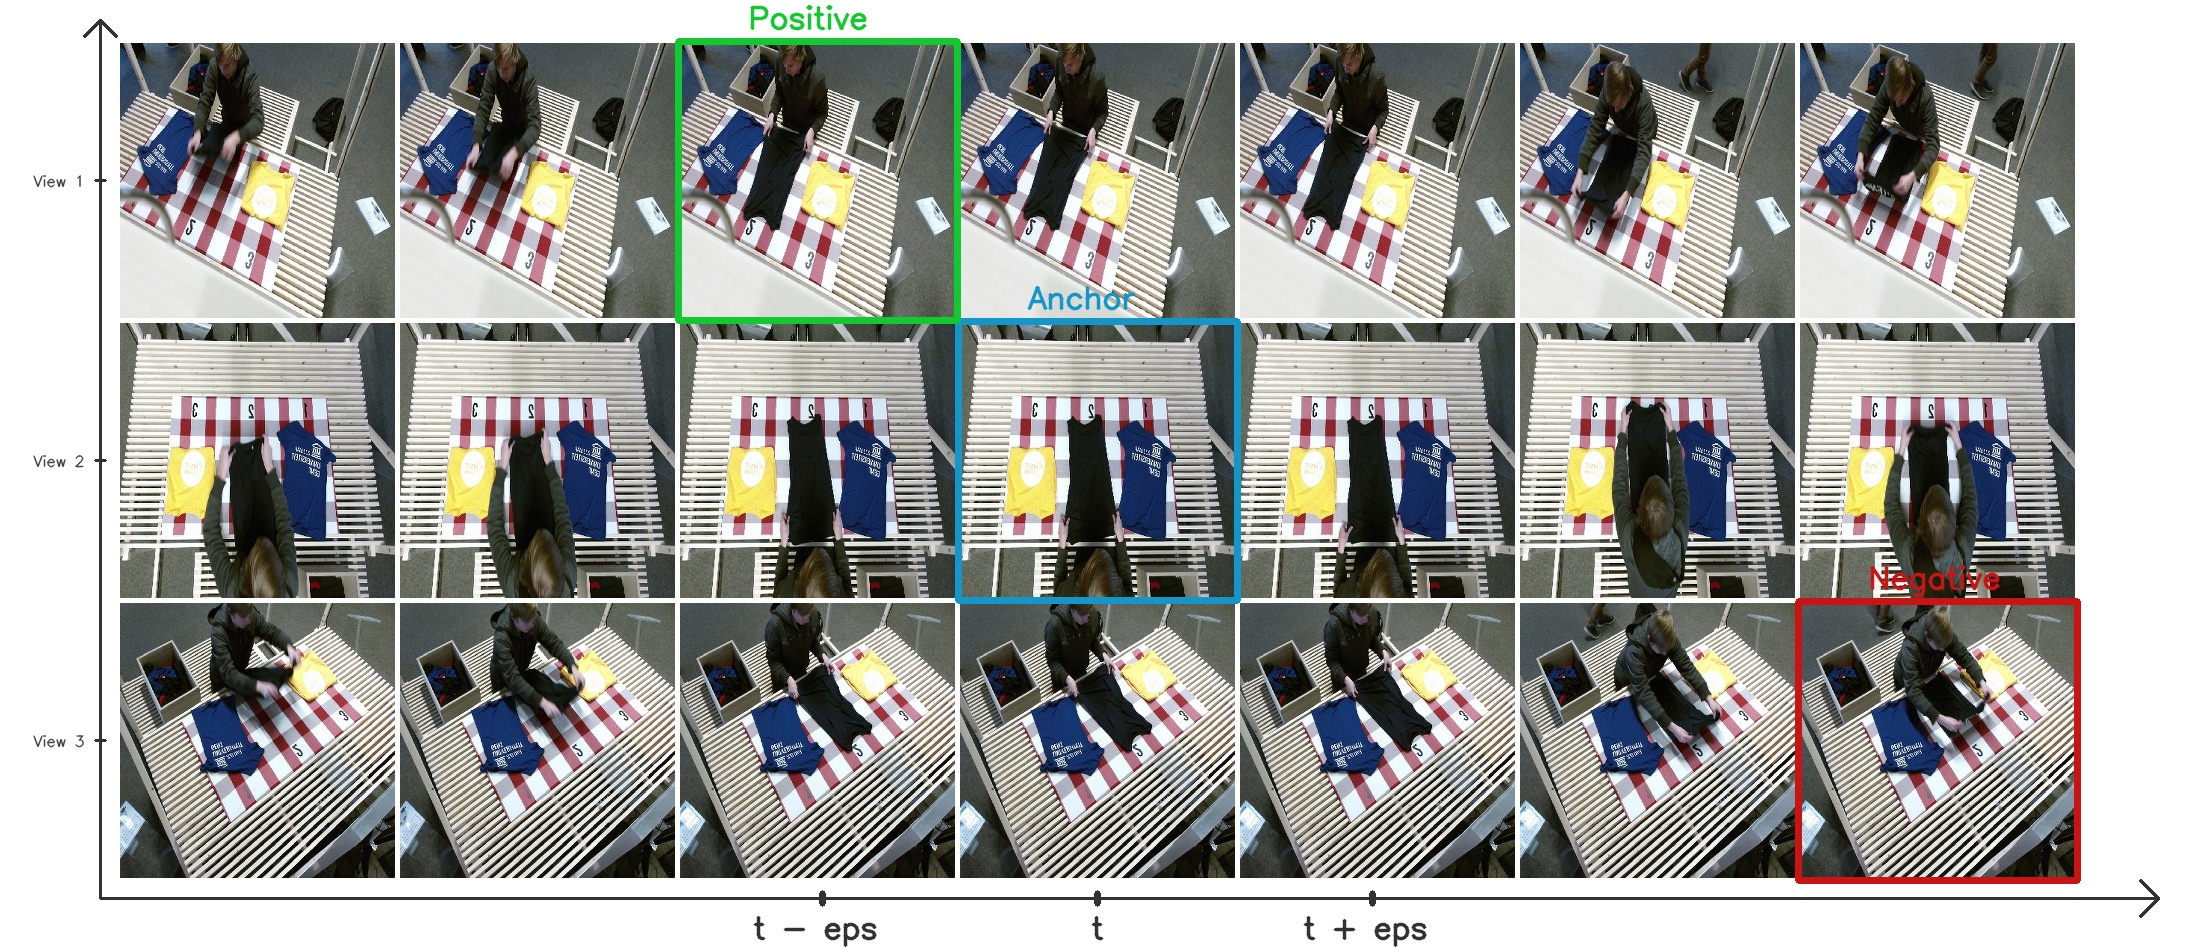
\includegraphics[width=\textwidth, keepaspectratio]{figures/figs_tcn_sampling.jpg}
    \caption[Principle of using time as a supervisory signal.]{\textbf{Using time as a supervisory signal in TCNs.} A randomly selected anchor frame (in blue) and a nearby temporal neighbour from a different perspective (in green) are encouraged to be close in the embedding space compared to the anchor frame and a distant temporal neighbour (in red). This allows the network to learn to explain changes in the physical world.}
    \label{fig:rewards_triplet_mining}
\end{sidewaysfigure}

\begin{algorithm}[htpb]
    \SetKwInOut{KwIn}{Input}

    \KwIn{training set of videos $\mathcal{V}$,\\
        temporal distance $\epsilon$,\\
        neural network $\tcn$ parametrized by $\theta$,\\
        margin $\alpha$,\\
        mini-batch size $k$}

    \ForEach{epoch}{

        $\text{loss} = 0$\;

        \For{$1$ \KwTo $k$}{
            select random video demonstration $v$ from $\mathcal{V}$ with frames $\mathcal{F}$\;
            select random anchor $a$ from $\mathcal{F}$\;

            generate positives $\mathcal{P} = \left\{ p \in \mathcal{V} : \temporalDist{(a, p)} \le \epsilon \right\}$\;
            find hardest positive $p^* = \argmax_{p \in \mathcal{P}} \left\{\euclDist{(\anchorEmbd, \positiveEmbd)}\right\}$\;

            generate negatives $\mathcal{N} = \left\{ n \in \mathcal{V} : \temporalDist{(a, n)} > \epsilon \right\}$\;
            generate semi-hard negatives $\mathcal{N}_{sh} = \left\{ n \in \mathcal{N}: \euclDist{(\anchorEmbd, \tcn{(p^*)})} < \euclDist{(\anchorEmbd, \negativeEmbd)}\right\} \cap \left\{n \in \mathcal{N}: \euclDist{(\anchorEmbd, \negativeEmbd)} < \euclDist{(\anchorEmbd, \tcn{(p^*)})} + \alpha \right\}$\;
            find easiest semi-hard negative $n^*$ with distance $\epsilon$ from $a$ with $n^* = \min_{n \in \mathcal{N}_{sh}} \left\{ \euclDist(\anchorEmbd, \negativeEmbd)\right\}$\;

            $\text{loss} \mathrel{+}= \euclDist(\anchorEmbd, \tcn{(p^*)}) - \euclDist(\anchorEmbd, \tcn{(n^*)}) + \alpha$\;
        }
        $\text{cost} = \text{loss} / k$\;
        Perform a gradient descent step on $\text{cost}$ with respect to the network parameters $\theta$ of the neural network $\tcn$\;
    }
    \caption{Training loop of time-contrastive network}
    \label{pseudocode:tcn}
\end{algorithm}

\subsection{Aligning expert video embeddings with query videos} \label{subsec:rewards_dtw}
% Structuur: 
%   Waarom DTW nodig, wat komt er in
%   Hoe werkt oorspronkelijk DTW -> grijp terug naar referentiewerk
%   Beschrijf aanpassingen dat we doen: move backwards in time + check impl

The TCN embedding trained in the previous section gives rise to a multivariate time series. In order to compare the time series embedding of a demonstrator $X = (x_1, \ldots, x_i, \ldots, x_N)$ to that of a chosen expert $Y = (y_1, \ldots, y_i \ldots, y_M)$ in order to judge the quality of the folding demonstration. To calculate the alignment between these time series, we use Dynamic Time Warping (DTW) \autocite{Bellman1959}. DTW is an algorithm for measuring the similarity between time series under time distortions. It minimizes the effects of shifting in time by allowing elastic transformations of the time series, subject to time-normalization constraints. This allows accounting for nonlinear task execution rate differences between two demonstrations. In DTW, an optimal path $P^*$ mapping time series $X$ and $Y$ are found:

% This is the previous notation where the time index was a subscript instead of variable
%\begin{align}
%    P^* = \argmin_{\phi_t, \psi_t} \sum_{t=1}^{\text{T}} d(x_{\phi_t}, y_{\psi_t}) \\
%\end{align}

\begin{subequations}
    \begin{alignat}{2}
         & \!P^* = \argmin_{\phi_x, \phi_y} & \qquad & \sum_{t=1}^{\text{T}} d(x_{\phi_x(t)}, y_{\phi_y(t)}),\nonumber\label{eq:of}
        %\\ TODO: we kunnen opteren om deze constraints voluit te schrijven
        %&\text{subject to} &      & \phi_x(1)=1,\nonumber\\
        %&                  &      & \phi_y(1)=1,\label{eq:startpoint}\\
        %&                  &      & \phi_x(T)=N,\nonumber\\
        %&                  &      & \phi_y(T)=M,\label{eq:endpoint}\\
    \end{alignat}
\end{subequations}
with $d()$ being a local distance function, for example, Euclidean distance. The alignment between the two time series is established through the mapping functions $(\phi_x(t), \phi_y(t))$. The warping functions are limited by certain constraints in order to be meaningful. Common warping constraints \autocite{Rabiner1993} are (1) start- and endpoint constraints as a clear start and end are manually specified by preprocessing the data, (2) monotonicity constraint which maintains temporal order during time normalization, and (3) local continuity constraints, also known as step patterns, to minimize loss of information. Compared to the canonical version of DTW, we relax the monotonicity constraint, which specifies that the alignment path does not go back in time. By allowing the time index of the expert time series $Y$ (i.e., the reference signal) to go back in time, we can account for demonstrators restarting part of the task execution or even executing the task backward. This also allows for coping with a failed task execution. We also relax the formulation to open-end DTW \autocite{Tormene2009} by removing the endpoint constraint to incorporate the possibility that demonstrators are not finishing the task optimally or completely. A visual interpretation on how we align a demonstration to video frames of an expert is given in \cref{fig:dtw}. We show the single component of two fictitious one-dimensional embeddings. The demonstration of which we need to calculate the task progression is labelled as the query. This is aligned to the embedding time series of the expert. The warping path is drawn in the global cost matrix. The coloured sections on the time series and alignment path represent subtasks. The background colours represent similar task progression or the same subtasks in the videos of the expert and query sample.

\begin{figure}[htbp]
    \centering
    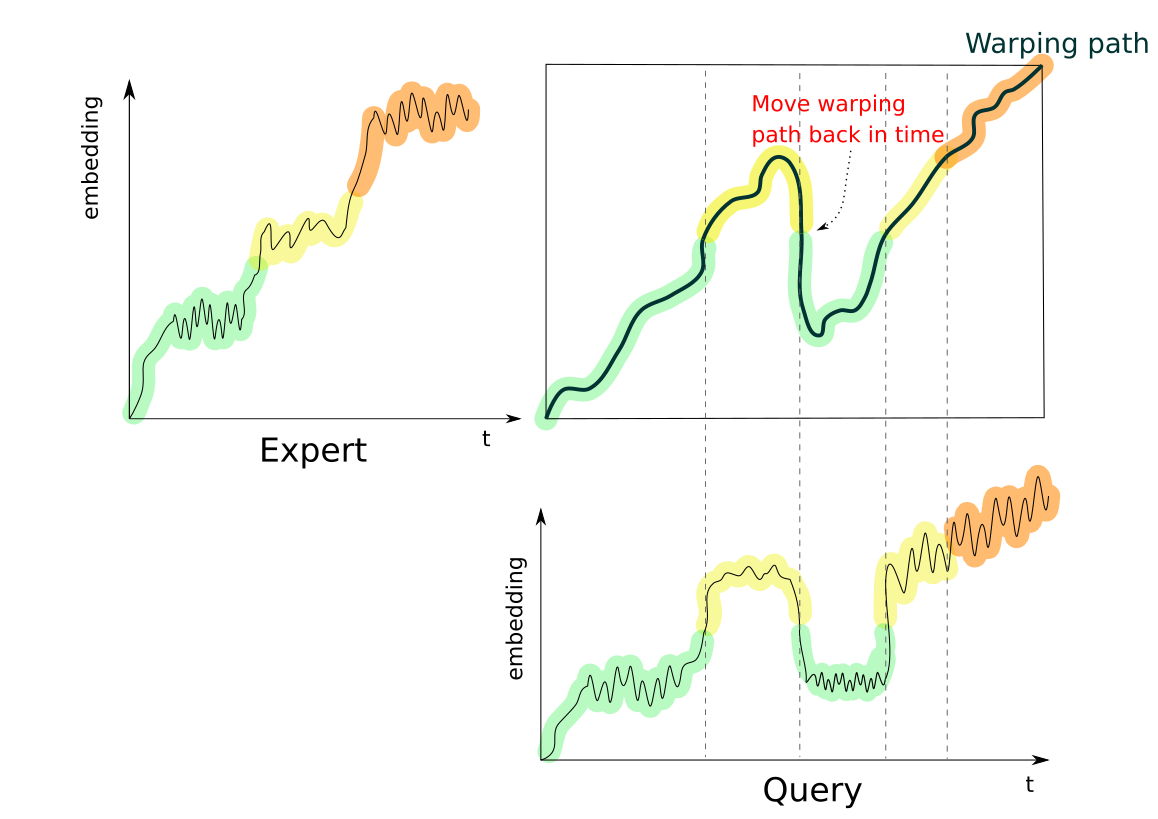
\includegraphics[width=0.90\textwidth, keepaspectratio]{figures/figs_dtw_backwards_v05.png}
    \caption[Dynamic Time Warping (DTW) without monotonicity constraint.]{\textbf{Dynamic Time Warping (DTW) without monotonicity constraint.} We align a multivariate time series embedding of a demonstration (the query) to the video frames of an expert. The time index is allowed to go back in time in order to correctly align a demonstration in which executed actions undo the made progress.}
    \label{fig:dtw}
\end{figure}

\subsection{Extracting task progression from embeddings} \label{subsec:rewards_extract}
The last step in our methodology is to extract task progression indicators using the aligned embeddings. First, we search which frame of each expert aligns best with each frame of the demonstration. The alignment score is expressed as the reciprocal of the cost of the best fit between them. Then, we select the temporal index of the best matching frame of every expert and express it as progress in percentage. Next, we average the experts' progress ratings by weighting with the normalized fit scores of the DTW phase of the pipeline. Finally, we remove any outliers by rejecting progress predictions of experts that deviate too much from the median of the absolute deviations \autocite{Leys2013}.

% ===================================================

\section{Results on folding clothing}\label{sec:rewards_results}
We use the multi-perspective dataset of people folding clothing collected and processed in \cref{ch:data_collection}.
We manually select \qty{5}{\percent} of the data as experts, which will later represent the signal to align other video demonstrations using DTW. This selection was based on two simple criteria: (1) the resulting fold looks successful, and (2) the demonstrator executes substeps to solve the task in one go. The last criterion implies that to go from an initial state to a target state, the fold is executed in one flow and not paused in between or divided into multiple intermediate states. The data contains multiple sources of randomization as the recordings took place at two different locations, of which one is a public library. This makes it useful to learn multiple invariances.

We first discuss quantitative results on training the embedding and extracting the reward functions. Afterwards, we conduct a qualitative assessment by inferring what the embeddings are encoding and testing the reward functions for specific adversary cases.

\subsection{Training results}

The first step in our methodology is to train TCNs using multiperspective images of task demonstrations. The neural network architecture we used is given in \cref{fig:rewards_nn_architecture}. We utilize the DenseNet \autocite{DenseNet2017} architecture pre-trained on ImageNet \autocite{ImageNet} as it already contains semantic relevant features for general-purpose vision-based tasks. Depending on the application, other neural network architectures can be used as a backbone. We append four trainable convolutional layers to the output of the DenseNet architecture. Afterwards, the output is passed to a spatial softmax layer \autocite{Levine2016}. The spatial soft arg-max layer produces the expected image-space positions of the points of maximal activations of the features in the former convolutional layer. This allows decoding of the relative position of salient objects in the scene. The spatial softmax layer is succeeded by two fully-connected layers of $2048$ and $32$ neurons. The neurons in the last layer represent the compact low-dimensional representation of the task execution, which we will use downstream to generate a task progression metric. We train the network for $500$ epochs using Adam optimization. Other fixed parameters during our experiments are given in \cref{table:rewards_settings}.

To tune the hyperparameters of our method, we split the dataset into a training, validation and test set. We define the split at the level of the demonstration and not at the collective set frames. This means that a validation and test sample is a complete, novel example demonstration of folding a piece of cloth. We define a range for each identified hyperparameter in \cref{table:rewards_hyperparams}. Then, we evaluate all possible combinations of the hyperparameters using the semi-hard triplet loss, amount of semi-hard triplets and the fraction of successful hard negatives. We explain these quantitative metrics in the next paragraph. Finally, we select the set of hyperparameters that performs best on these training metrics on the validation set. The test set is used for the subsequent steps of translating the learned embedding to a scalar progression value. We provide the final hyperparameters used in our experiments in \cref{table:rewards_hyperparams}.

\begin{figure}[htb]
    \centering
    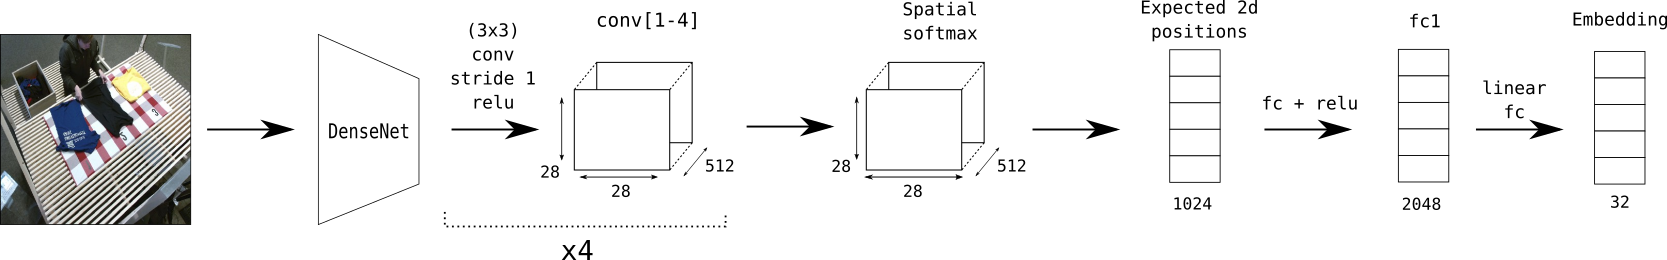
\includegraphics[width=0.90\textwidth, keepaspectratio]{figures/figs_ssr_nn_architecture.png}
    \caption{
        \textbf{Neural network architecture.} We use a pre-trained DenseNet backbone appended with four trainable convolutional layers. It is followed by a spatial softmax layer, which produces the expected 2D coordinates of the region of maximal activation in each channel of conv4. These coordinates are manipulated by a fully connected layer, which is finally passed through to the compressed embedding space.
    }
    \label{fig:rewards_nn_architecture}
\end{figure}

\begin{table}[htbp]
    \centering
    \caption{Fixed settings during training of the TCN embedding.}
    \begin{tabular}[t]{@{} l r @{}}

        \toprule
        Hyperparameter        & Value                   \\
        \midrule
        Optimizer             & Adam                    \\
        Weight initialization & Glorot initialization   \\
        \# Epochs             & $500$                   \\
        Image size            & $224 \times 224$ pixels \\
        GPU                   & $1$ NVIDIA Quadro P6000 \\
        \bottomrule
    \end{tabular}
    \label{table:rewards_settings}
\end{table}

\begin{sidewaystable}
    \centering
    \caption{Hyperparameters used for learning an embedding to extract task progression metrics for folding clothing items.}
    \begin{tabular}[t]{@{} l c c @{}}

        \toprule
        Hyperparameter                                               & Best value                    & Value range                                                                                     \\
        \midrule
        Learning rate                                                & $0.001$                       & $\left[ 0.0001, 0.001, 0.01, 0.1 \right]$                                                       \\
        Batch size                                                   & $32$ samples                  & $\left[ 16, 32, 64 \right]$                                                                     \\
        Embedding dimension                                          & $32$ neurons                  & $\left[ 16, 32, 64 \right]$                                                                     \\
        \makecell{Max temporal distance between anchor and positive} & $3\mskip\thinmuskip \text{s}$ & $0.5\mskip\thinmuskip \text{s}$,  $1\mskip\thinmuskip \text{s}$,  $3\mskip\thinmuskip \text{s}$ \\
        Margin                                                       & $0.2$                         & $\left[0.1, 0.2, 0.4, 0.8 \right]$                                                              \\
        NN backbone                                                  & DenseNet                      & VGG, ResNet, DenseNet                                                                           \\

        \bottomrule
    \end{tabular}
    \label{table:rewards_hyperparams}
\end{sidewaystable}

In \cref{fig:rewards_tcn_training_metrics}, we show quantitative results of training the TCN. The loss quickly and steadily improves, as visible in \cref{fig:rewards_semihardtripletloss}. This indicates that transfer learning from the DenseNet backbone advances smoothly. However, the semi-hard triplet mining strategy presents more difficult training triplets over time to the network. This might result in oscillating loss functions making it necessary to monitor additional metrics. In particular, we monitor the amount of semi-hard triplets still available in the batches and the percentage of successful hard negatives. \cref{fig:rewards_semihardtriplets} shows that pushing a new semi-hard negative out of the margin does not lead to an increased amount of new semi-hard triplets re-entering the margin. \cref{fig:rewards_successfulhardnegatives} examines which fraction of the \textit{anchor-hardest positive} pairs are closer in embedding space compared to the \textit{anchor-hardest negative} pairs. This metric steadily increases, indicating that meaningful clusters are formed in embedding space to temporally separate images from different viewpoints.


\begin{figure}[p]{}
    \centering
    \begin{subfigure}[b]{0.95\textwidth}
        \centering
        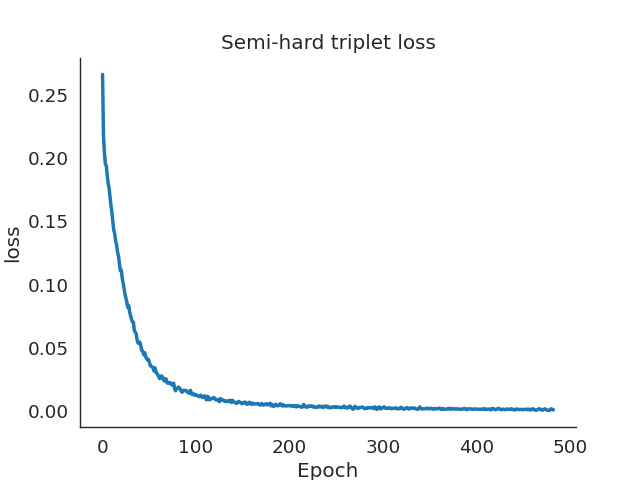
\includegraphics[width=\linewidth]{figures/figs_plots_semi-hard-triplet-loss.png}
        \caption{Semi-hard triplet loss}
        \label{fig:rewards_semihardtripletloss}
    \end{subfigure}

    \vskip\baselineskip

    \begin{subfigure}[t]{0.45\textwidth}
        \centering
        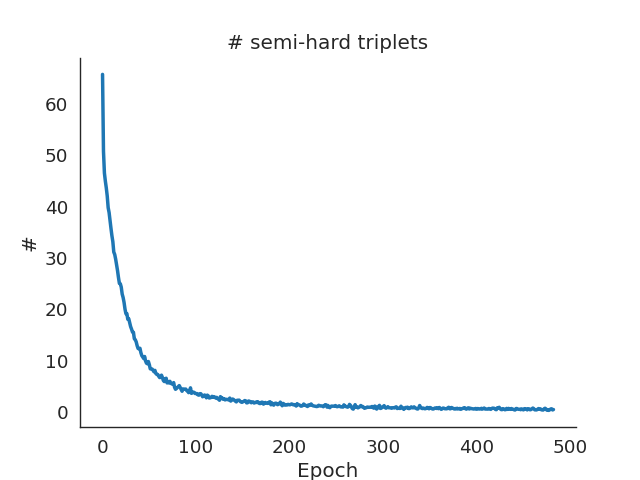
\includegraphics[width=\linewidth]{figures/figs_plots_semi-hard-triplets.png}
        \caption{Amount of semi-hard triplets}
        \label{fig:rewards_semihardtriplets}
    \end{subfigure}
    \hfill
    \begin{subfigure}[t]{0.45\textwidth}
        \centering
        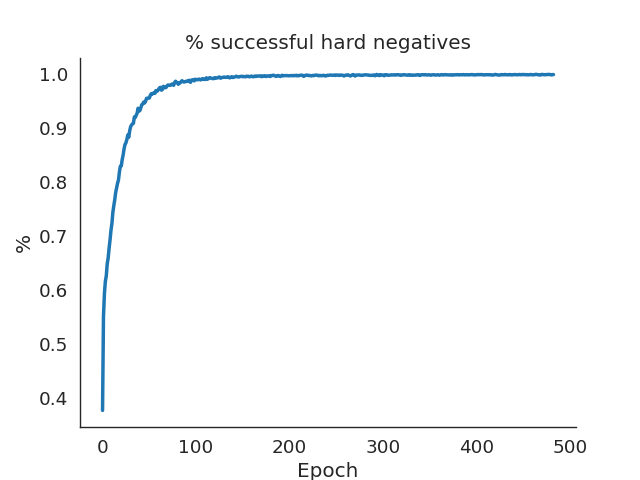
\includegraphics[width=\linewidth]{figures/figs_plots_succesful-hard-negatives.png}
        \caption{Percentage of hard negatives successfully separated}
        \label{fig:rewards_successfulhardnegatives}
    \end{subfigure}

    \caption{Loss and training metrics of the TCN training process with semi-hard triplet loss as optimization objective.}
    \label{fig:rewards_tcn_training_metrics}
\end{figure}


\subsection{Reward function results}
We align the resulting embeddings using DTW as described in \cref{subsec:rewards_dtw}. We use a symmetric stepping pattern \autocite{Rabiner1993} with a maximum step size up to 10~frames, corresponding with approximately 1~second. \cref{fig:rewards_reward_plot} shows the task progression, or reward function, of a sample in the dataset. We annotated points in the plot with the corresponding image in the video demonstration. This shows that the task progression metric increases at meaningful moments in the demonstration. For example, when the demonstrator grasps the shirt to unfold on the table, the progression score increases from \qty{0}{\percent} to \qty{40}{\percent}. Afterwards, the progression scalar value stagnates because the demonstrator slowly moves the right sleeve to the middle. Once the sleeve is folded, the progression indicator climbs. Next, the demonstrator grabs the left part of the shirt relatively quickly and moves it to the centre. This action is reflected in the progression value raising more quickly compared to the previous fold. Finally, the demonstrator receives maximum progression on completely folding the shirt. We find these results to be consistent among samples in the dataset. We provide videos of the task progression metric of other samples on \url{https://youtu.be/_HJhn8Hbv5s}. The whole pipeline requires $63\mskip\thinmuskip \text{ms}$ to process a single frame, with the slowest step being the alignment.

\begin{sidewaysfigure}
    \centering
    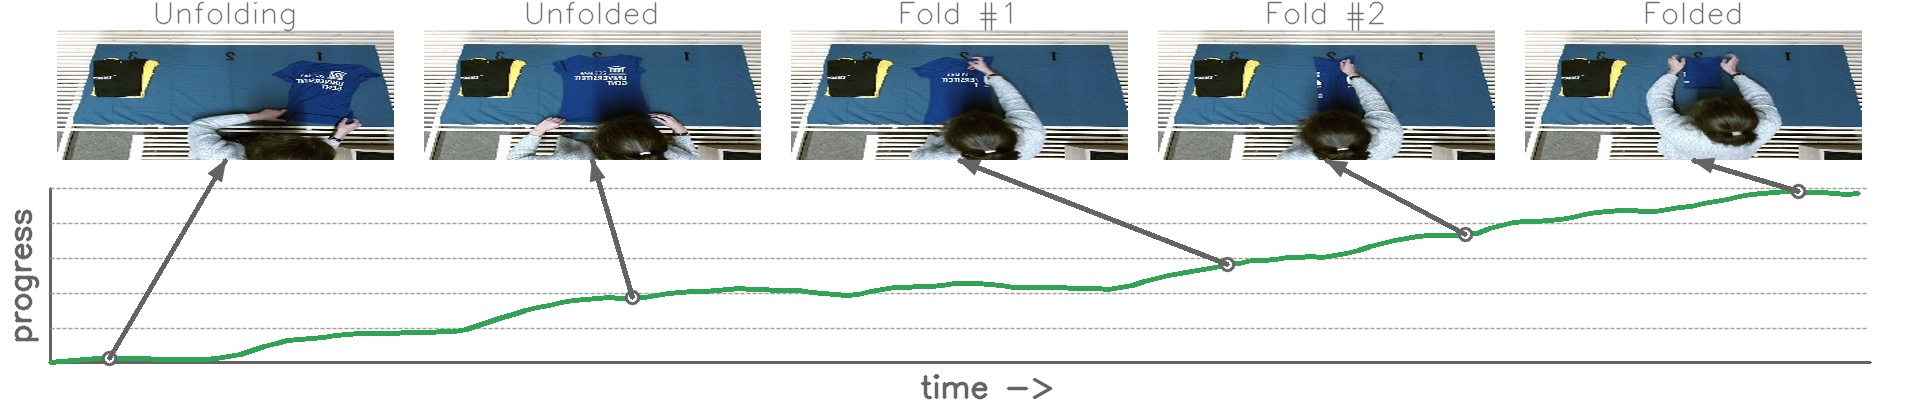
\includegraphics[width=\textwidth,keepaspectratio]{figures/figs_cases_paper_reward_plot_383.jpg}
    \caption[Task progression plot with corresponding video frames of a single demonstration]{\textbf{Task progression plot with corresponding video frames of a single demonstration.} Each image is annotated with what is happening in the scene.}
    \label{fig:rewards_reward_plot}
\end{sidewaysfigure}

In conclusion, we find training of the embeddings in a self-supervised manner to be stable and efficient by using a semi-hard triplet function loss where we push out the easiest hard cases out of the margin first. Aligning the resulting embeddings with DTW on manually selected reference samples and using the alignment to express task progression increases progression scores on meaningful moments in the demonstration. This suggests that the embeddings encode task-relevant features. We analyze to which extent the embedding encodes important features for folding clothing in the next section.

% ===================================================

\section{Discussion}\label{sec:rewards_discuss}
In the previous section, we have shown that TCN embeddings can be temporally aligned to extract useful task progression metrics. We now analyze the embeddings for post hoc interpretability. The goal is to discover which semantics are learned from the input images. However, neural networks lack decomposability into intuitive and understandable components. This is why we leverage the following two methods to understand what the network is encoding. First, we look at the semantic meaning of the embeddings at multiple temporal levels in \cref{subsec:semantic meaning}. Second, we employ a case-based reasoning approach to interpret the learned representations and run robustness tests in \cref{subsec:rewards_cases}.

\subsection{Semantic Meaning of Learned TCN Embeddings}\label{subsec:semantic meaning}
To discover the encoded semantics in the learned representations, we examine how the embedding progresses over time while linking it to what is happening in the scene. First, we examine how the embedding changes during the progress of a demonstration. To make the visualization interpretable, we project it to a lower dimension. Second, we examine whether we can extract meaningful information when searching for clusters in latent space.

To qualitatively analyze the results of training the embedding, we project the $32$D embedding space to $2$D using UMAP \autocite{UMAP}. In \cref{fig:umap_111} we plotted the resulting projection mapped to the corresponding frame at different time shots. The time index is indicated with the colour of the scatter plot: from magenta to red, yellow, green, and blue.

A reoccurring observation is the projection of the embedding jumping at meaningful moments during task progression. In \cref{fig:umap_111}, we notice that while grasping the shirt from the pile, the embedding stays in the first quadrant. Once the shirt is unfolded on the table, the embedding jumps to quadrant two. During the execution of the required folding steps, the embedding jumps to other locations. For example, the embedding gently transitions from quadrant two to three when folding the right and left sleeves. This suggests that the embedding can recognize different substeps in the folding task. When performing the final fold, the embedding is positioned between the first and fourth quadrant. We find this observation to be consistent among other samples. Consequently, the embedding at the start and the end of a trial is very similar. The explanation can be found in the observations starting and ending with a pile of unfolded shirts on the right side of the table and a pile of folded shirts on the left side. A similar start and end encoding in embedding space imply that the network potentially has problems distinguishing the start and end of the trial from a single image when there is no notion of memory.

Another observation is the embedding following a trajectory to go from grasping a piece of unfolded clothing to completely folding it on the table. Given that, in general, the third quadrant encodes folding the shirt's sleeves, it is possible that folding methods that do not fold the sleeves will not be assigned the correct progression score as there is no alignment available. In other words, for the DTW alignment to work, there needs to be a trajectory followed in embedding space in order to arrive at the solution. We explore this in \cref{subsec:rewards_cases}.

\begin{figure}[!htbp]
    \centering
    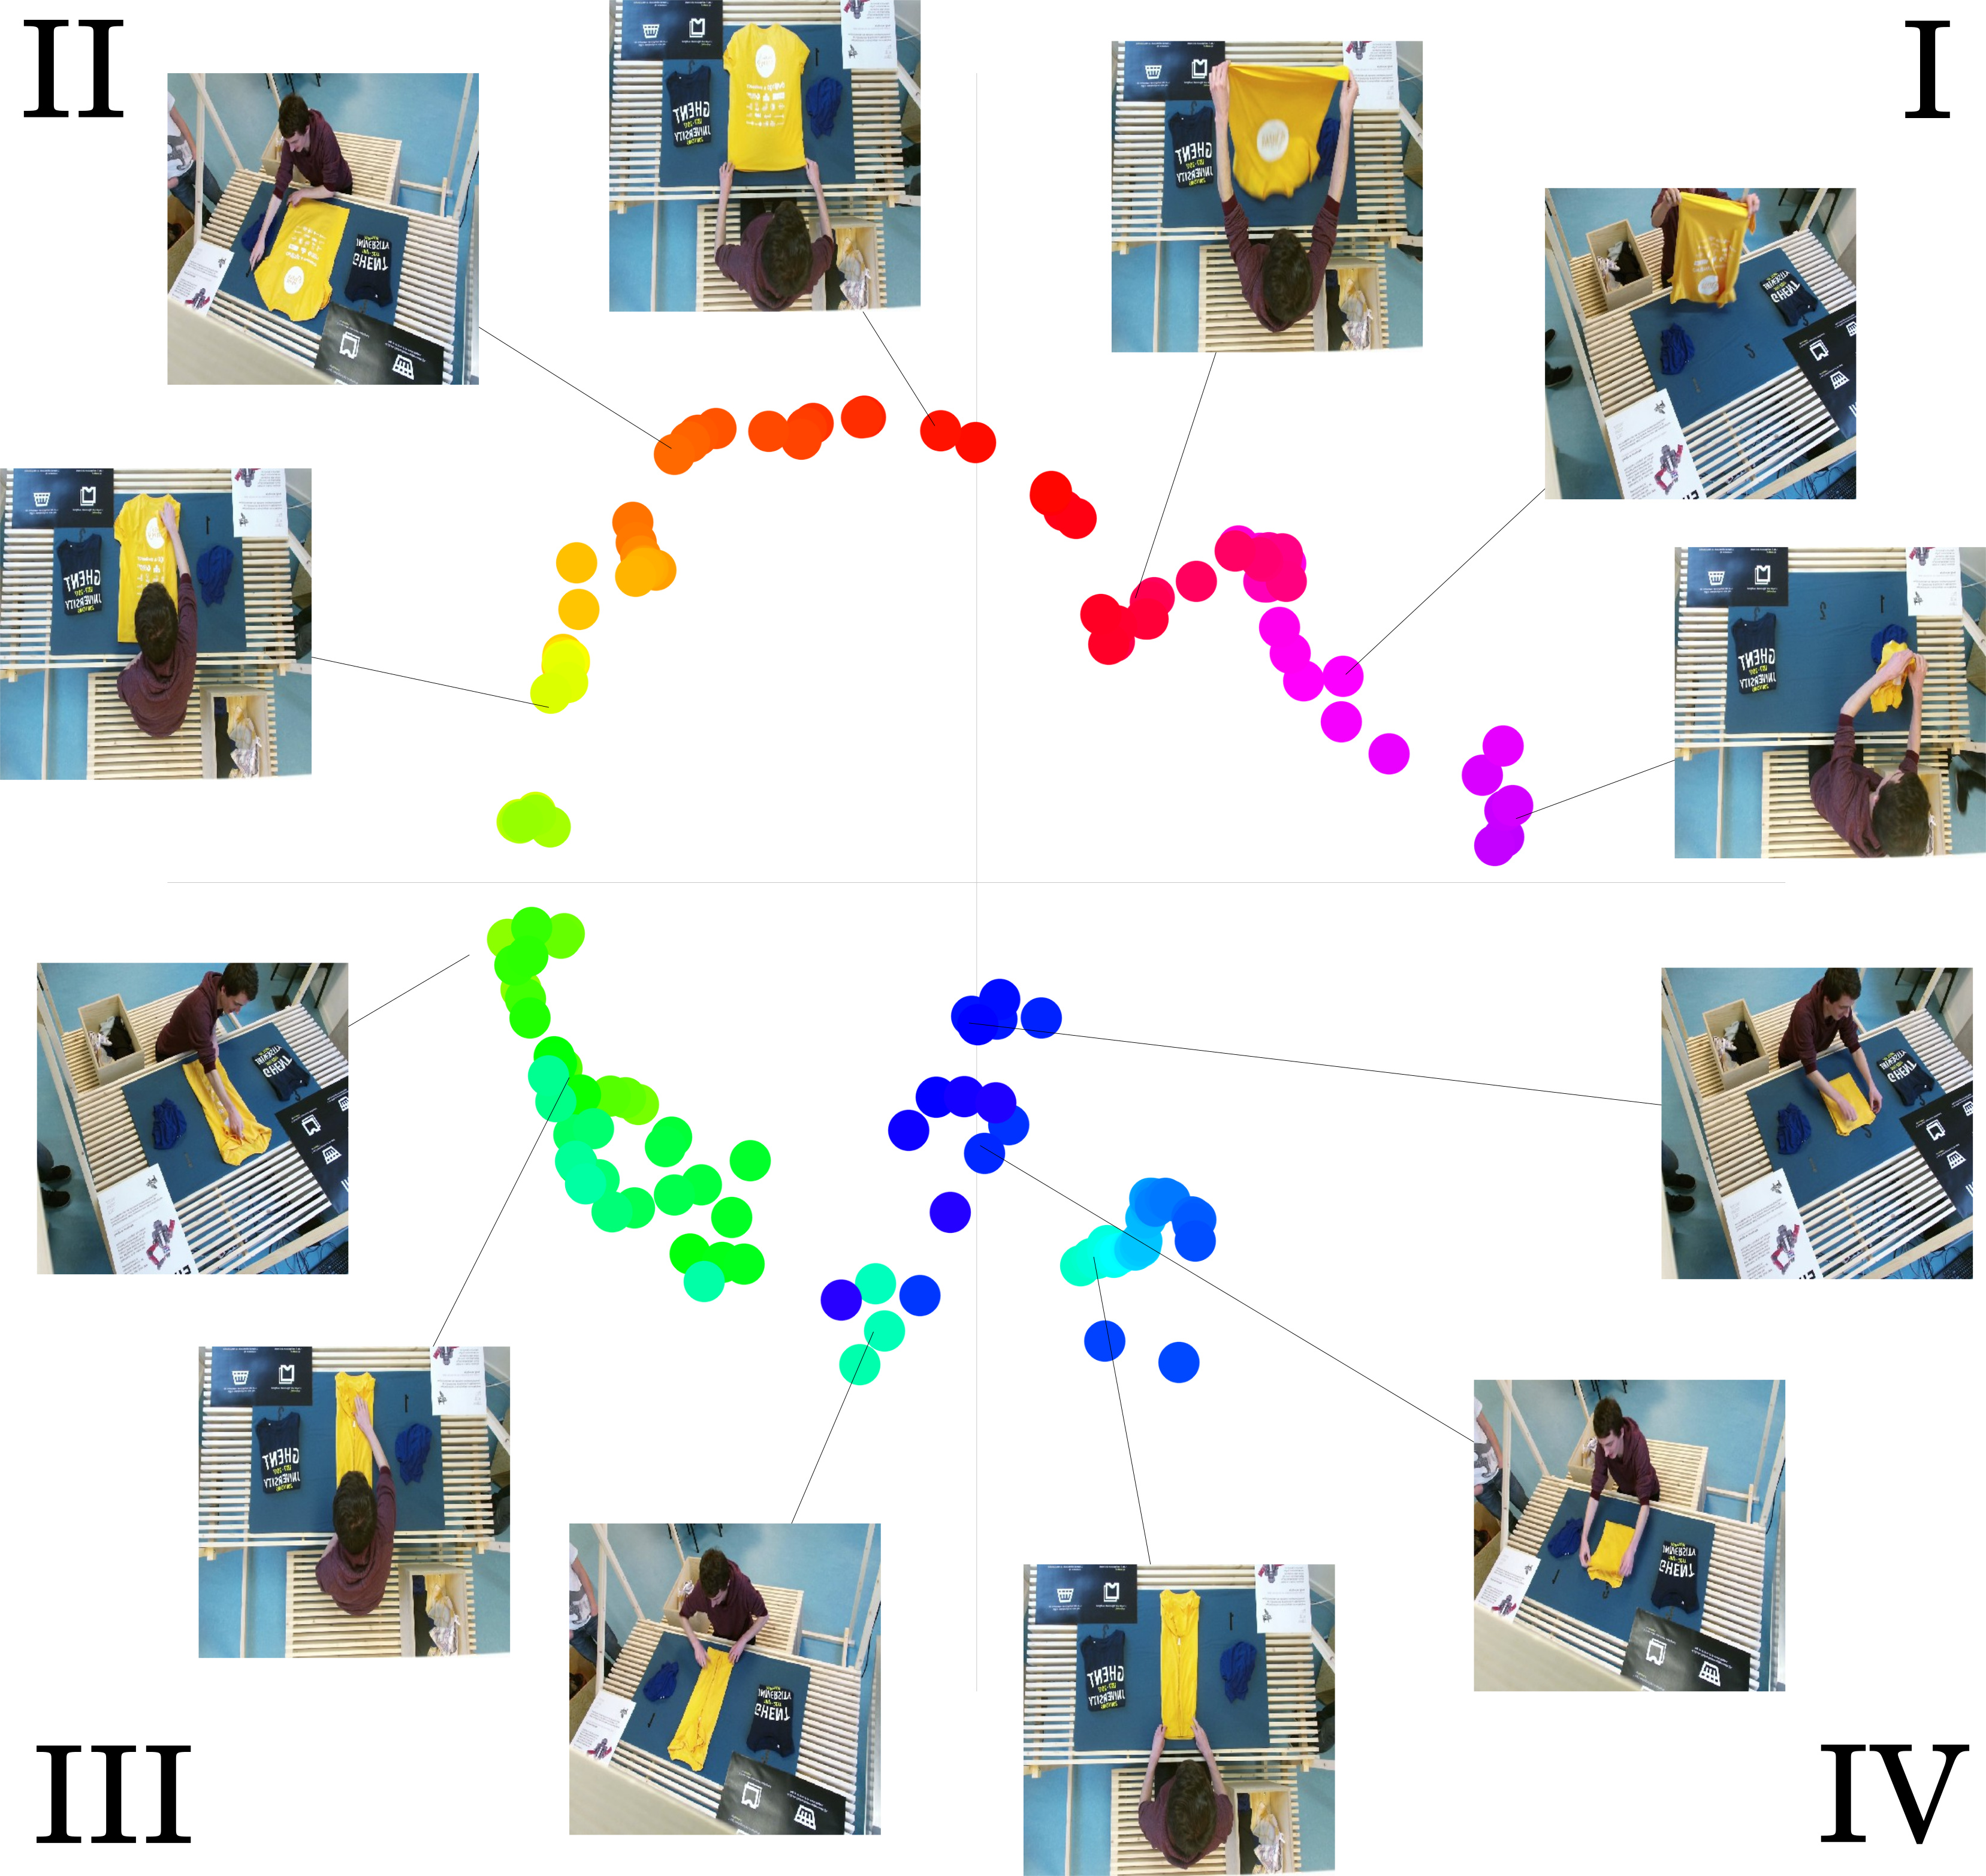
\includegraphics[width=\textwidth, keepaspectratio]{figures/figs_discussion_umap_111.jpg}
    \caption[2D projection of the learned TCN embedding]{\textbf{2D projection of the learned embedding.} We annotate some points in the quadrants with the corresponding images to offer insight in to what is happening in the scene. Colors in the scatter plot indicate time progression from magenta to yellow, green and finally to blue. }
    \label{fig:umap_111}
\end{figure}

To further analyze whether the embedding can distinguish meaningful moments during task execution, we generate clusters in the embedding hyperspace. We perform agglomerative clustering with ward linkage on each demonstration separately. Because our data is temporally sorted, we set the connectivity matrix as a square matrix with ones on the superdiagonal and subdiagonal, and zeros elsewhere. This way, we enforce the bottom-up cluster formation to consider temporal neighbours, reflecting the temporal ordering. We select five clusters to identify as they reflect the substeps in the task: grasping, flatten, fold one side, fold another side, fold in the middle. We visualize the results of the clustering in \cref{fig:wt_572}. Here, we show the 2D projection of using UMAP on the embedding, with the colour representing the cluster membership instead of the temporal dimension. Qualitatively, we find the emergence of subtasks in the cluster membership when running agglomerative clustering in embedding space. The task starts in quadrant I in the projected embedding space. This is indicated with the red cluster membership. Once the demonstrator unfolds the shirt on the table, the cluster membership switches to green while the embedding transitions towards quadrant II. The same process repeats when transitioning between the other subtasks. This indicates that the embedding encodes relevant aspects of the task, which downstream algorithms can use. However, we have no guarantees that the network picks up other signals from the environment during training. For example, the network might be encoding the position of the hands, or the size of the shirt. We examine which features the network is attending to in the following subsection.

\begin{figure}[!htbp]
    \centering
    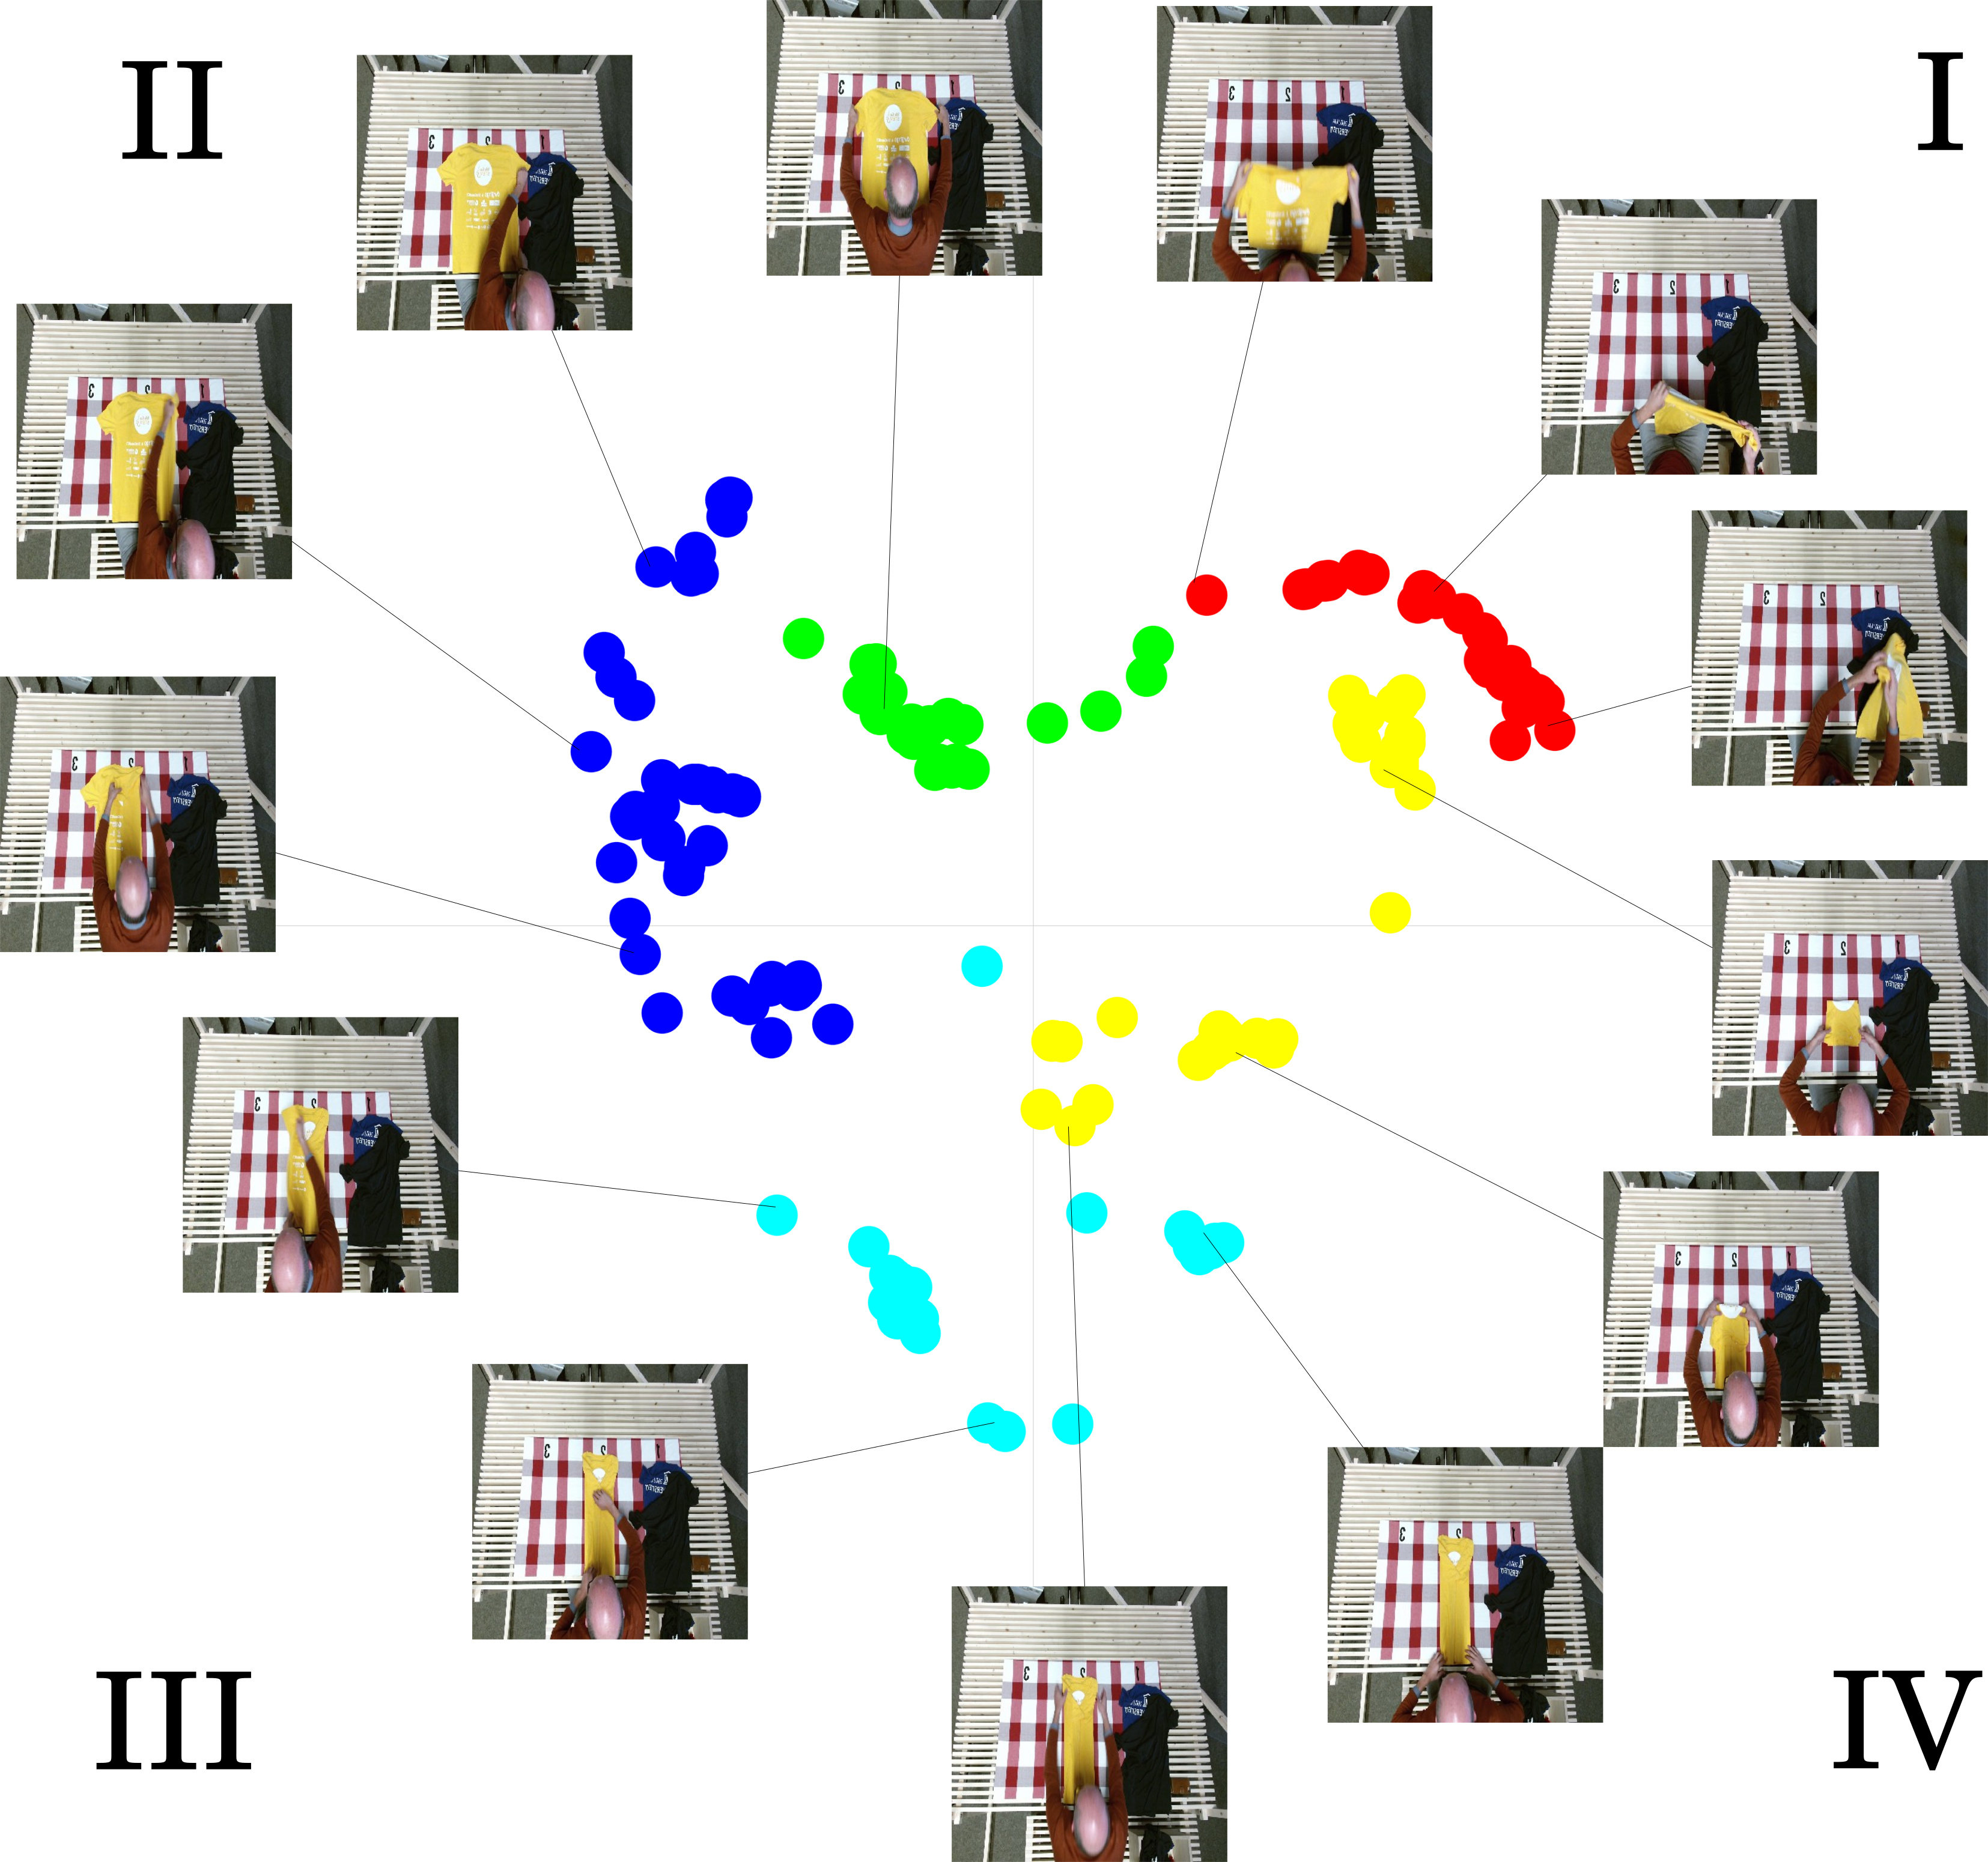
\includegraphics[width=\textwidth, keepaspectratio]{figures/figs_discussion_wt_572.jpg}
    \caption[Interpretation of embedding using agglomerative clustering]{\textbf{Interpretation of embedding using agglomerative clustering.} Colors in the scatterplot indicate cluster membership. One point in the scatterplot represents an embedded video frame, projected onto a 2D plane using UMAP. The line links images to the corresponding embedding.}
    \label{fig:wt_572}
\end{figure}

\subsection{Case-based examples for post hoc interpretability} \label{subsec:rewards_cases}

For the learned task progression metrics to be useful, they must be able to capture and generalize to specific situations that arise during the execution of the task, not seen in the training set. For example, a task executor can be performing random manipulations without actually performing meaningful contributions towards progressing the given task. This is also the case for learning purposes; many RL algorithms start with an exploration phase in which the robot acts randomly. To research the generalizability of our method, we employ a case-based approach in which we input certain scenarios and qualitatively analyze the result of our pipeline. We first describe the relevant scenario, followed by the resulting task progression scores, and offer insight into why a specific scenario succeeds or fails. \cref{fig:casesP1} and \cref{fig:casesP2} contains the visualizations of the cases we discuss below. We annotated the plotted task progression with specific frames from the demonstration to explain changes in the assigned progression. Videos of these hold-out samples are available at \url{https://youtu.be/ZvK0pQWH8ec}.

\paragraph{Change of environment with background distractions.}
Practical reasons and safety concerns make it possible that workers perform the designed process flow in another environment compared to the demonstrators. To test whether the learned progression metric can cope with this, we set up the folding table in a location not seen during training and fold clothing while putting random objects on the table. The images corresponding to the annotated parts of the plotted task progression in \cref{fig:casesP1a} show that adding distractor objects such as a safety helmet, a flashlight, and a quadruped robot, do not prevent the learned task progression metric from assigning a correct progression score. There are two potential reasons for this. First, the data is recorded in a public environment where distractions are inherently present. Second, the TCNs are forced to attend high-level, task-relevant features. This filters out distractions in the image.

\paragraph{Meaningful manipulations compared to random behavior.}
Non-meaningful, random manipulations in the process execution occur in both process monitoring and scenarios where agents are learning to solve a task. Because fully random behaviour is not present in the data provided by the crowdsourced demonstrations, it is uncertain how the learned progression metric associate this with process quality. We explore how the progression metric evolves by first doing a meaningful manipulation of the shirt, followed by randomly moving the hands above the shirt. This experiment is displayed in \cref{fig:casesP1b}. We find that the progression metric correctly assigns an intermediate score on unfolding the shirt. For the subsequent random movement of the arms of the demonstrator, no additional progress is made according to the metric. In similar experiments where demonstrators move their arms without any shirts on the table, we noticed that the network tries to distil meaningful manipulations. For example, a frequently reoccurring movement is performing the final fold where demonstrators grab the shirt at the bottom and fold it to the top. In some of those cases, we notice that the progression score increases due to the trajectory of the hands being recognized. However, the progression correctly drops again when the network detects that there is no shirt being folded. We explore this further in the next paragraph.

\paragraph{Attention to the essence of the task.}
In the previous paragraph, we examined the effect of random behaviour on the learned task progression metric. Here we compare non-meaningful behaviour to meaningful manipulations to test to which extent the neural network is paying attention to the essence of the task. We do this by setting up a scenario to test to which extent the neural network looks at the hand trajectories while monitoring the state of the textile. Concretely, we try to fool the network: we first solve a subtask and then execute the required arm trajectories to solve the task but without touching the clothing. We hypothesize that in case the embedding is solely looking at the executed trajectories and not the clothing, the assigned task progression will increase. The result in \cref{fig:casesP1c}. shows that the progression value increases when the shirt is unfolded. It is followed by stagnation of the progression score because the demonstrator is not manipulating the clothing. This demonstrates that our method looks at task-relevant features, like the state of the clothing, to indicate task progression. \emph{This feature is what sets our method apart from behavioural cloning}; our method searches for the essence of the task instead of imitating end-effector trajectories.

\paragraph{Different task execution speed.}
The resulting progression metric should cope with different task execution speeds resulting from using different demonstrating entities. Given our crowdsourced dataset, this issue is already present in the training data. It is solved by aligning the resulting embedding time series with DTW. We verify that this is working as intended by performing the folds of a shirt at different speeds. We provide the results of this experiment in \cref{fig:casesP1d}. We label the start and end of the folds in order to indicate the different speeds at which the task is solved. For example, the first fold is executed rapidly, leading to a quick increase in task progression values. Contrary, the second fold is executed by moving the right sleeve very slowly to the centre of the shirt. Once the sleeve is folded, a sudden increase in task progression is given.

\paragraph{Different task executor morphology.}
Industrial processes can be performed by any human actor or machine. In order for the learned progression metric to be useful, it has to generalize across actors with different morphologies. We test this by folding the shirt with two people, such that four arms are manipulating the clothing. The results, visible in \cref{fig:casesP1e}, show that the resulting progression metric behaves correctly. This demonstrates that our trained embedding is invariant to the actor executing the task.

\paragraph{Variations in task execution.}
Task progression metrics should cope with different variations in executing the task. We test this in multiple ways: we fold the task by lying out the shirt diagonally, undo, and repeat some of the substeps and doing excessive wrinkle flattening. We find that the given progression value is correct and consistent in all these scenarios. In particular, we examine the case in which a shirt is folded and then unfolded again. The unfolding is executed by the demonstrator and not by playing the video in reverse. The resulting task progression, visible in \cref{fig:casesP1f}, shows that the maximum progression is reached when the shirt is folded. When the demonstrator starts undoing the fold step by step, the task progression correctly drops. This hold-out sample demonstrates that our alignment step does not contain an upward drift. This is important as the training data only exist of successful folds, leading to alignments that primarily run from start to end of the anchor and demonstrator. Hence the DTW step extracts useful information from the embedding to cope with failing task executions.

\paragraph{Generalization towards other folding methods.}
In extension to examining how well the learned task progression metric copes with variations on task execution, we look at how well they generalize when unseen folding methods are used. We test the case in which the demonstrator uses an alternative, unseen folding method where folds are executed on the table and in the air. In \cref{fig:casesP2a}, we find that the assigned progression increases while folds are realized. We notice that the progression score suddenly drops on the step \textit{unfolded square} (annotated in grey font above the corresponding image). By looking at the embeddings, as demonstrated in \cref{subsec:semantic meaning}, we find that is due to the embedding state transitioning to the \textit{unfolded} step. Afterwards, the progression correctly increases to the maximum level while performing the last folding steps.
We also test the case when folding only two steps instead of four. The results of this experiment are visible in \cref{fig:casesP2b}. In this case, the process monitoring metric only detects the folded shirt very late in the folding process. The explanation can be found in the training data: the experts have never seen folding solutions with four steps. Given that the alignment process expects a certain trajectory to be followed in embedding space, the alignment fails.

\paragraph{Generalization towards other instances of the target object.}
We introduce shirts with other colours, textures, and reflective material to investigate how well our method generalizes to other shirt instances. We provide an example demonstration of a shirt with reflective material in \cref{fig:casesP2c}. Reflective objects are known to cause problems for object recognition neural networks \autocite{sajjan2019cleargrasp}. In this case, the learned process monitoring metric detects increasing progression on meaningful moments when solving the task. One instance in which the progression metric did not react appropriately is when folding tiny shirts, for example, in \cref{fig:casesP2d}. When increasing the size of the shirt to normal proportions, the progression metric starts behaving appropriately. We hypothesize this is due to the embedding not reacting to very small hand movements and changes in the shirt, which lead to small pixel value changes in the image.

\paragraph{Task quality.}
We investigate to which degree the learned process monitoring metric incorporates the quality of the end result. We do this by examining how the task progression evolves when small and large disruptions are made in the resulting fold of the shirt. In \cref{fig:casesP2e}, we disarrange the end fold of the shirt considerably. This leads to the demonstrator not achieving the maximum task progression at the end of the episode because the sleeves are partly hanging out of the shirt. However, in the experiment visualized in \cref{fig:casesP2f}, we apply a small perturbation of the folded shirt, which is not picked up by the process monitoring metric. We find that a rectangular folded shape with many wrinkles receives the same progression score as a perfectly flattened one. This can potentially be solved by using cameras closer to the shirt, using depth information to incorporate wrinkles in the embedding, or manually constructing triplets of end results with good and bad flattening. \\

To summarize, we find that our method captures meaningful events in the task by looking at relevant features in the scene. By examining the assigned task progression values on the discussed hold-out samples, we show that the learned process monitoring metric is invariant to the demonstrator's morphology, background scene, execution speed and distractions. Our method is largely invariant to the shirt being manipulated, except that when the shirt gets too small, the resulting folds are not detected. Additionally, our method is not fooled by performing the expected arm trajectories without actually folding the shirt. We notice that the maximum progression value achieved during a successful folding demonstration consistently corresponds to the end-fold of the shirt. However, it is not possible to make meaningful comparisons in the end-quality of the fold of different demonstrations. We find meaningful reactions to highly visible disruptions in the shirt, but not to small wrinkles and small imperfections in the fold. In general, we find that the learned process monitoring metric effectively captures task progression and small degrees of output quality.

\begin{figure}[p]
    \centering
    \begin{subfigure}[b]{\linewidth}
        \begin{minipage}{0.94\linewidth}
            \centering
            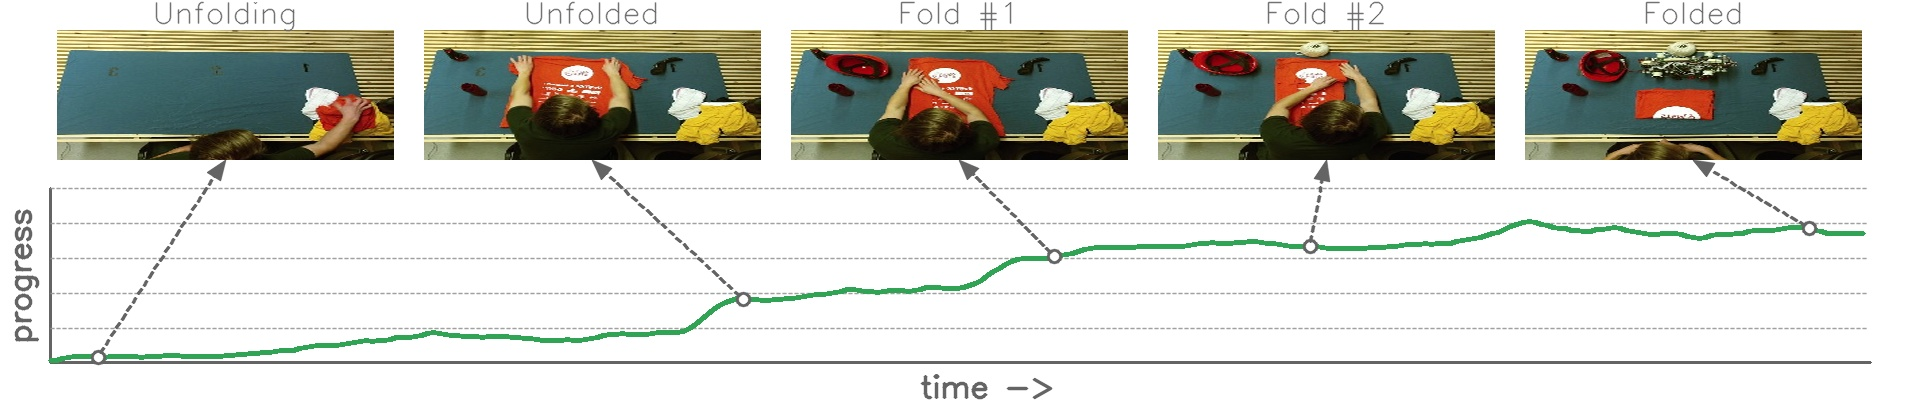
\includegraphics[width=\linewidth]{figures/figs_cases_paper_reward_plot_1019.jpg}
        \end{minipage}
        \begin{minipage}{0.04\linewidth}
            \caption{}
            \label{fig:casesP1a}
        \end{minipage}
    \end{subfigure}

    \par\medskip

    \begin{subfigure}[b]{\linewidth}
        \begin{minipage}{0.94\linewidth}
            \centering
            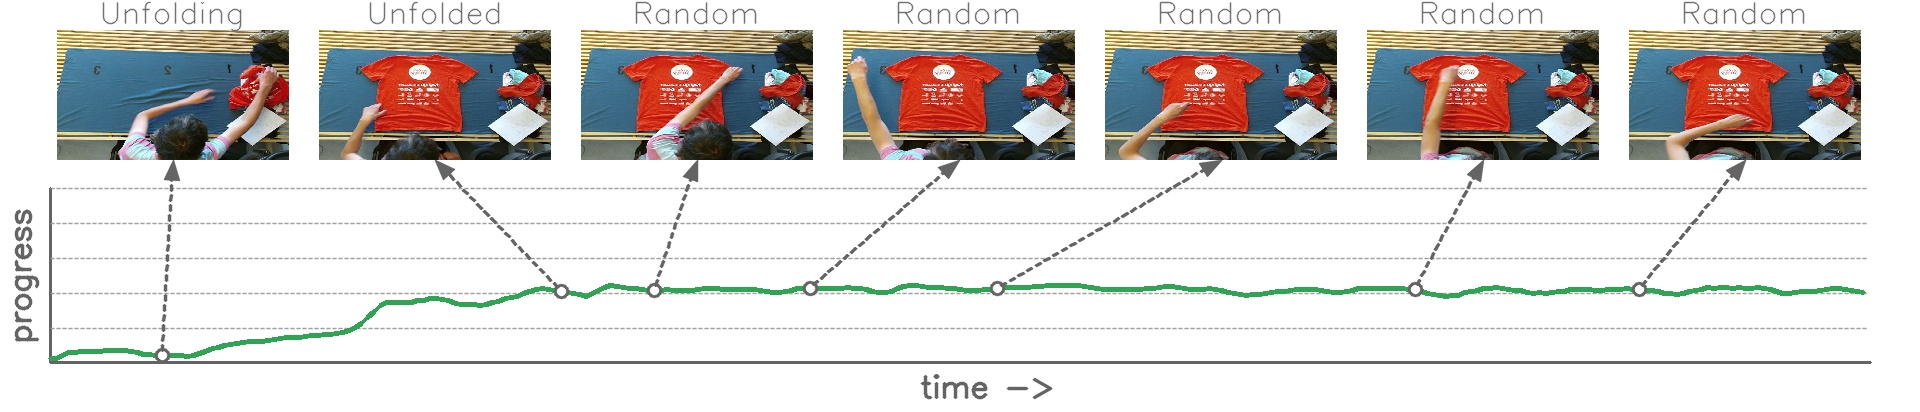
\includegraphics[ width=\linewidth]{figures/figs_cases_paper_reward_plot_1125.jpg}
        \end{minipage}
        \begin{minipage}{0.04\linewidth}
            \caption{}
            \label{fig:casesP1b}
        \end{minipage}
    \end{subfigure}

    \par\medskip

    \begin{subfigure}[b]{\linewidth}
        \begin{minipage}{0.94\linewidth}
            \centering
            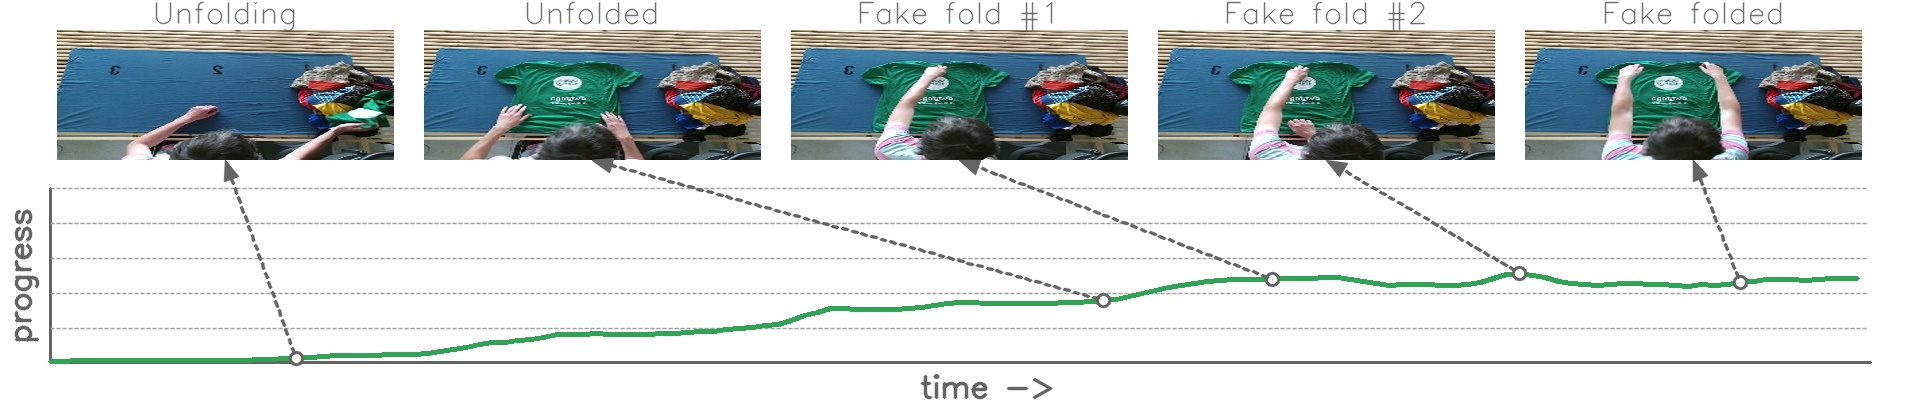
\includegraphics[ width=\linewidth]{figures/figs_cases_paper_reward_plot_1110.jpg}
        \end{minipage}
        \begin{minipage}{0.04\linewidth}
            \caption{}
            \label{fig:casesP1c}
        \end{minipage}
    \end{subfigure}

    \par\medskip

    \begin{subfigure}[b]{\linewidth}
        \begin{minipage}{0.94\linewidth}
            \centering
            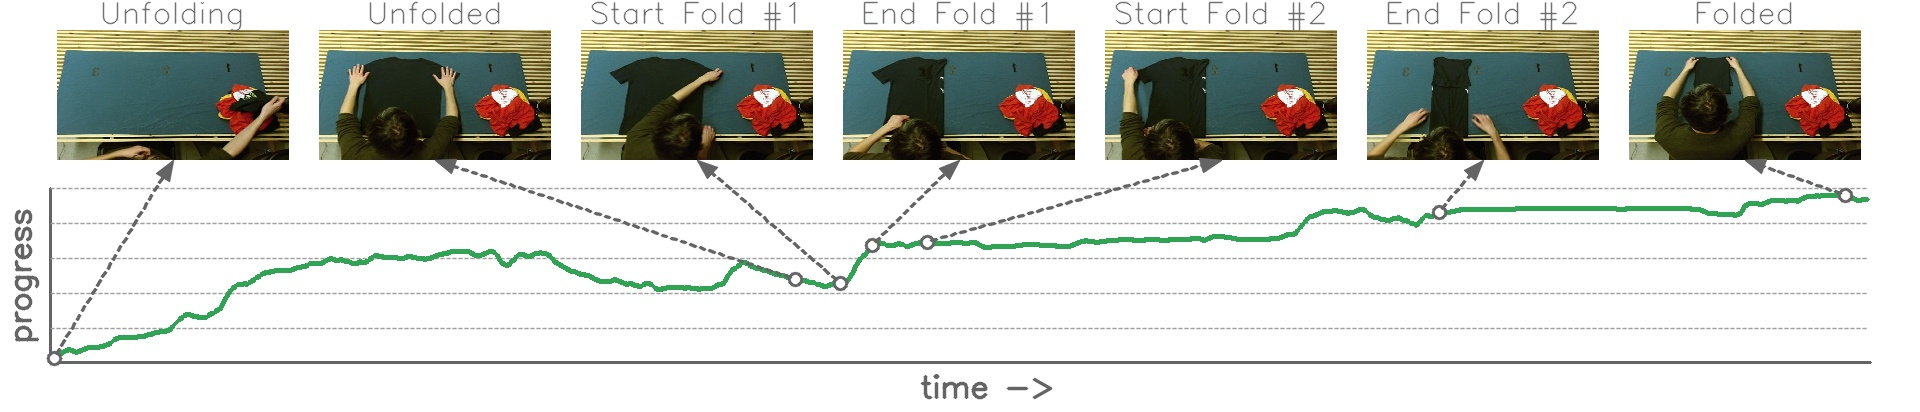
\includegraphics[ width=\linewidth]{figures/figs_cases_paper_reward_plot_1004.jpg}
        \end{minipage}
        \begin{minipage}{0.04\linewidth}
            \caption{}
            \label{fig:casesP1d}
        \end{minipage}
    \end{subfigure}

    \par\medskip

    \begin{subfigure}[b]{\linewidth}
        \begin{minipage}{0.94\linewidth}
            \centering
            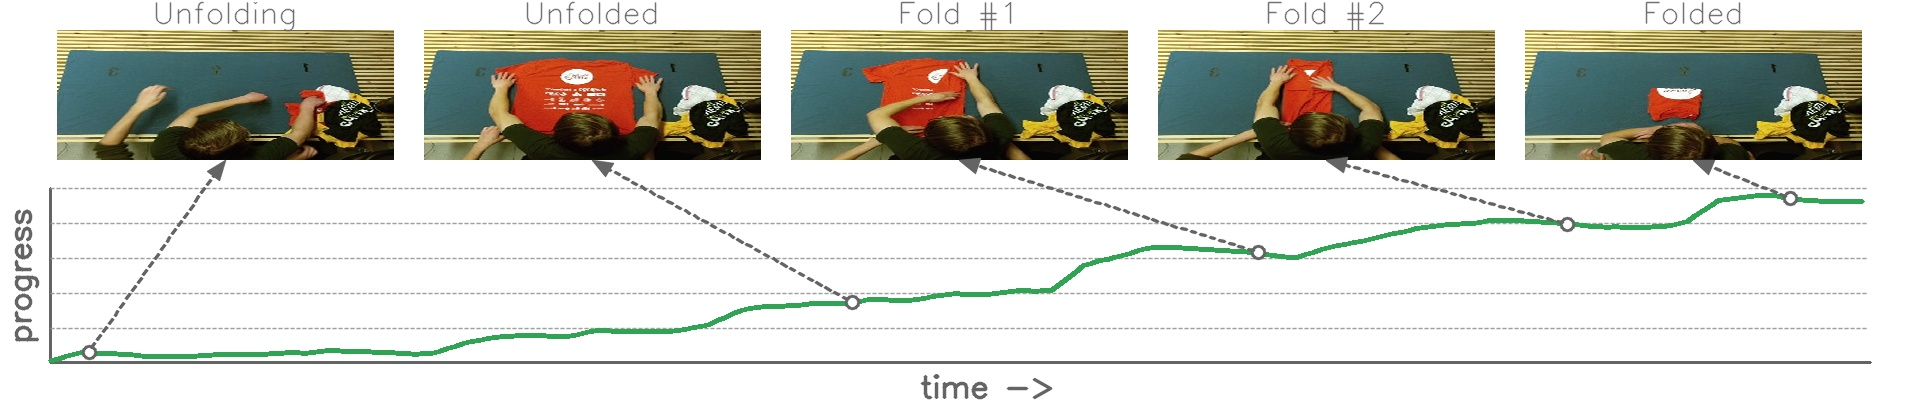
\includegraphics[ width=\linewidth]{figures/figs_cases_paper_reward_plot_1021.jpg}
        \end{minipage}
        \begin{minipage}{0.04\linewidth}
            \caption{}
            \label{fig:casesP1e}
        \end{minipage}
    \end{subfigure}
    \par\medskip

    \begin{subfigure}[b]{\linewidth}
        \begin{minipage}{0.94\linewidth}
            \centering
            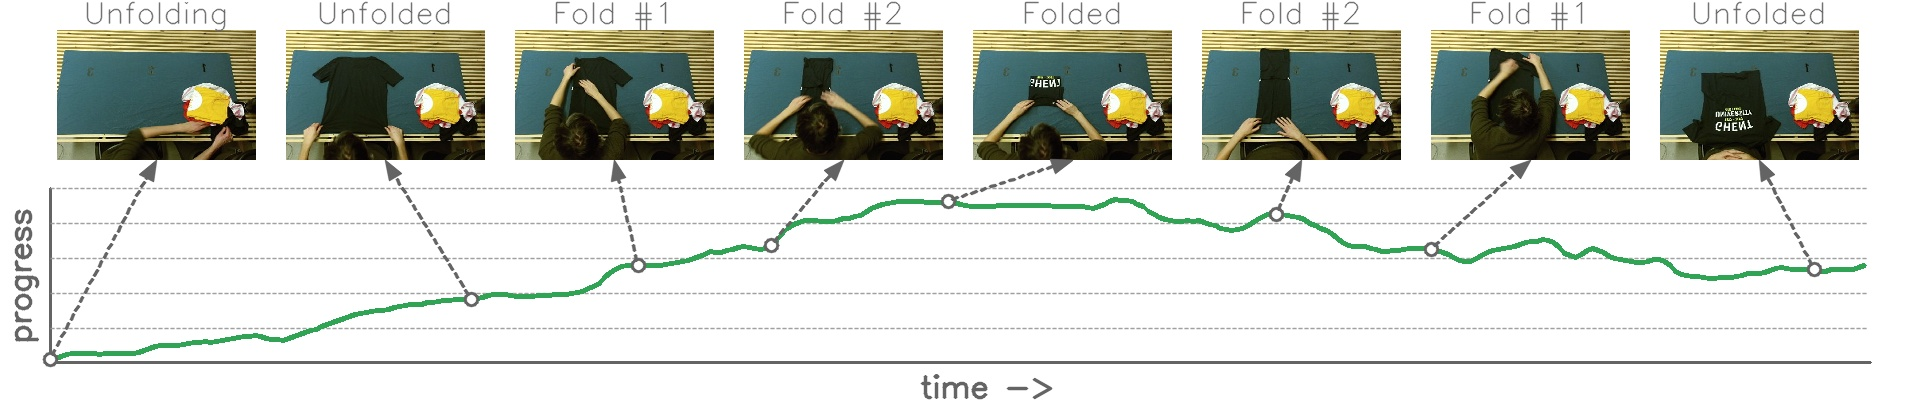
\includegraphics[ width=\linewidth]{figures/figs_cases_paper_reward_plot_1029.jpg}
        \end{minipage}
        \begin{minipage}{0.04\linewidth}
            \caption{}
            \label{fig:casesP1f}
        \end{minipage}
    \end{subfigure}

    \caption{Task progression plots and corresponding images of out-of-sample cases to specifically test properties of the learned process monitoring metrics.}
    \label{fig:casesP1}
\end{figure}

\begin{figure}[p]
    \centering
    \begin{subfigure}[b]{\linewidth}
        \begin{minipage}{0.94\linewidth}
            \centering
            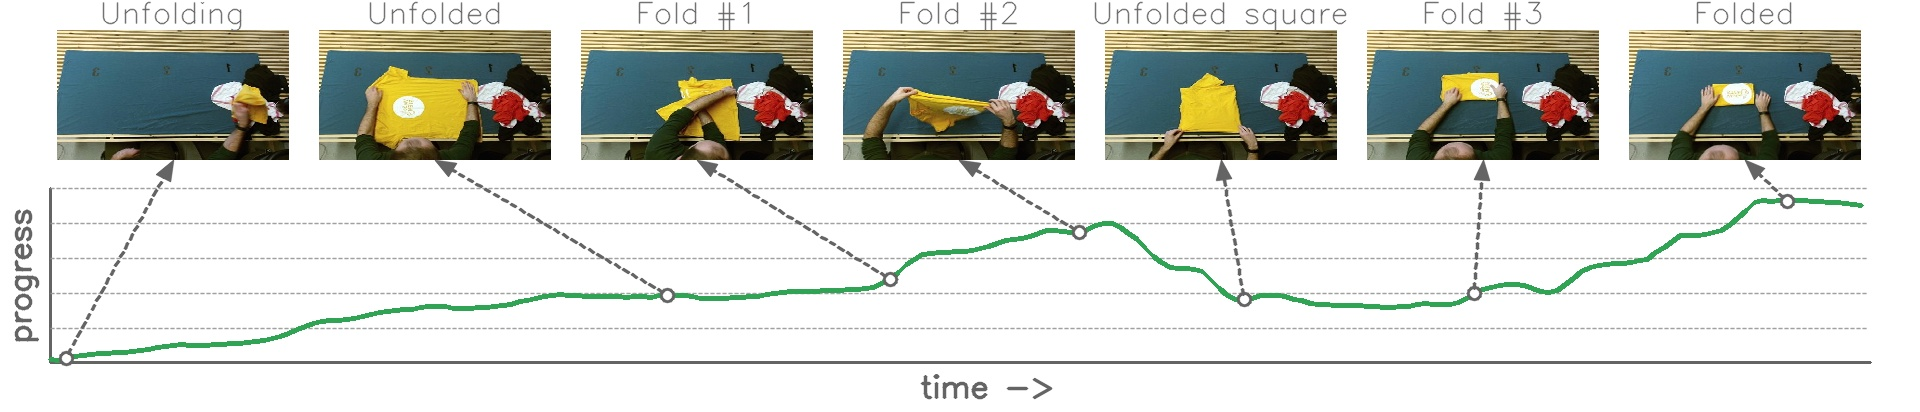
\includegraphics[width=\linewidth]{figures/figs_cases_paper_reward_plot_1035.jpg}
        \end{minipage}
        \begin{minipage}{0.04\linewidth}
            \caption{}
            \label{fig:casesP1a}
        \end{minipage}
    \end{subfigure}

    \par\medskip

    \begin{subfigure}[b]{\linewidth}
        \begin{minipage}{0.94\linewidth}
            \centering
            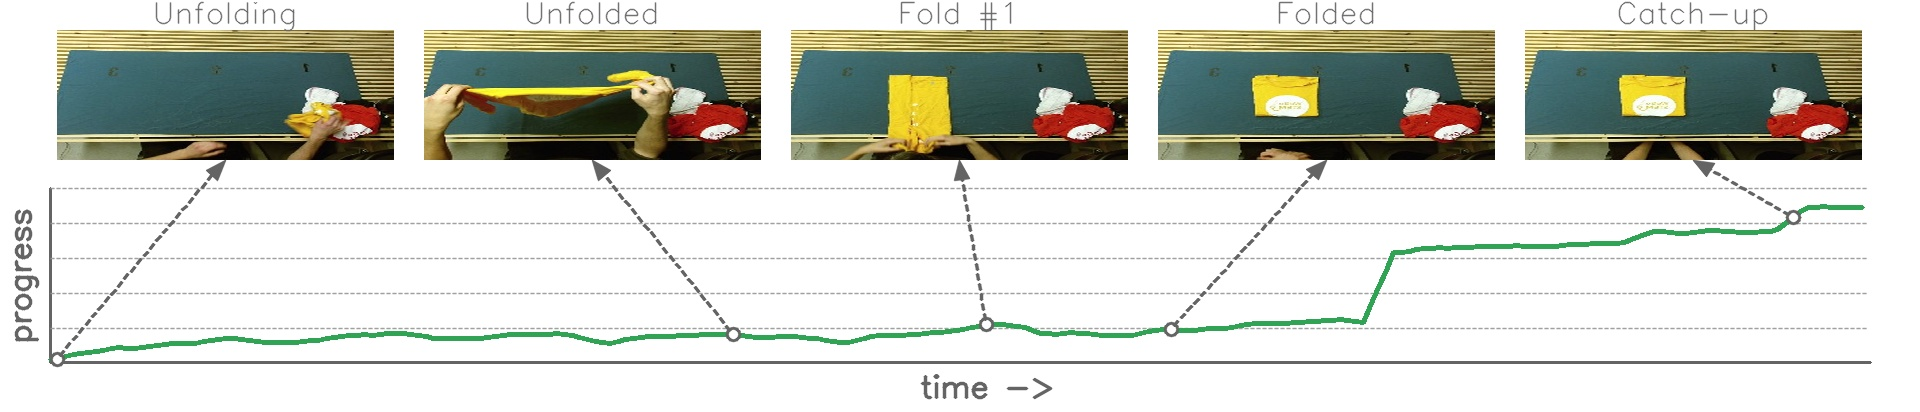
\includegraphics[ width=\linewidth]{figures/figs_cases_paper_reward_plot_1015.jpg}
        \end{minipage}
        \begin{minipage}{0.04\linewidth}
            \caption{}
            \label{fig:casesP1b}
        \end{minipage}
    \end{subfigure}

    \par\medskip

    \begin{subfigure}[b]{\linewidth}
        \begin{minipage}{0.94\linewidth}
            \centering
            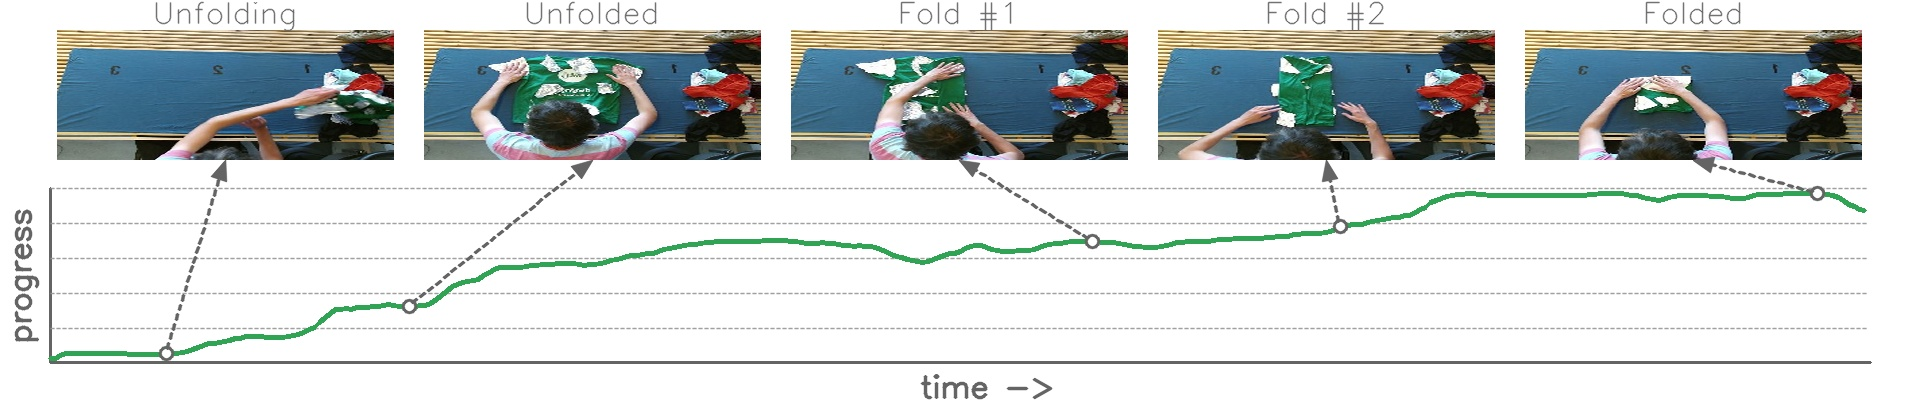
\includegraphics[ width=\linewidth]{figures/figs_cases_paper_reward_plot_1118.jpg}
        \end{minipage}
        \begin{minipage}{0.04\linewidth}
            \caption{}
            \label{fig:casesP1c}
        \end{minipage}
    \end{subfigure}

    \par\medskip

    \begin{subfigure}[b]{\linewidth}
        \begin{minipage}{0.94\linewidth}
            \centering
            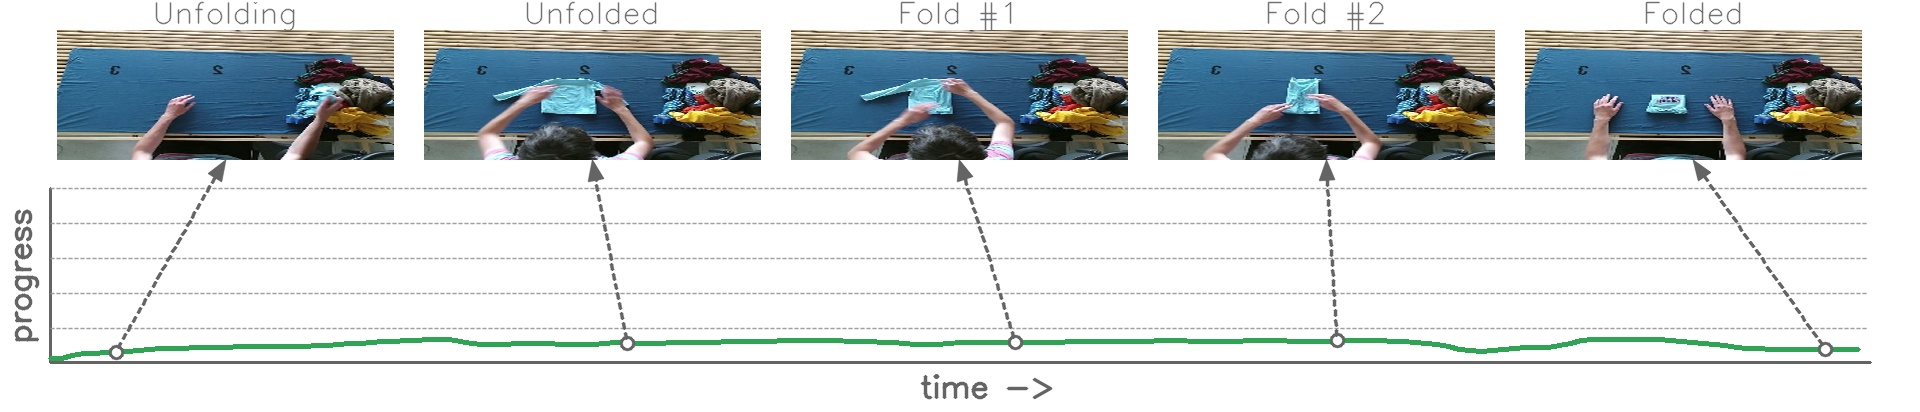
\includegraphics[ width=\linewidth]{figures/figs_cases_paper_reward_plot_1103.jpg}
        \end{minipage}
        \begin{minipage}{0.04\linewidth}
            \caption{}
            \label{fig:casesP1d}
        \end{minipage}
    \end{subfigure}

    \par\medskip

    \begin{subfigure}[b]{\linewidth}
        \begin{minipage}{0.94\linewidth}
            \centering
            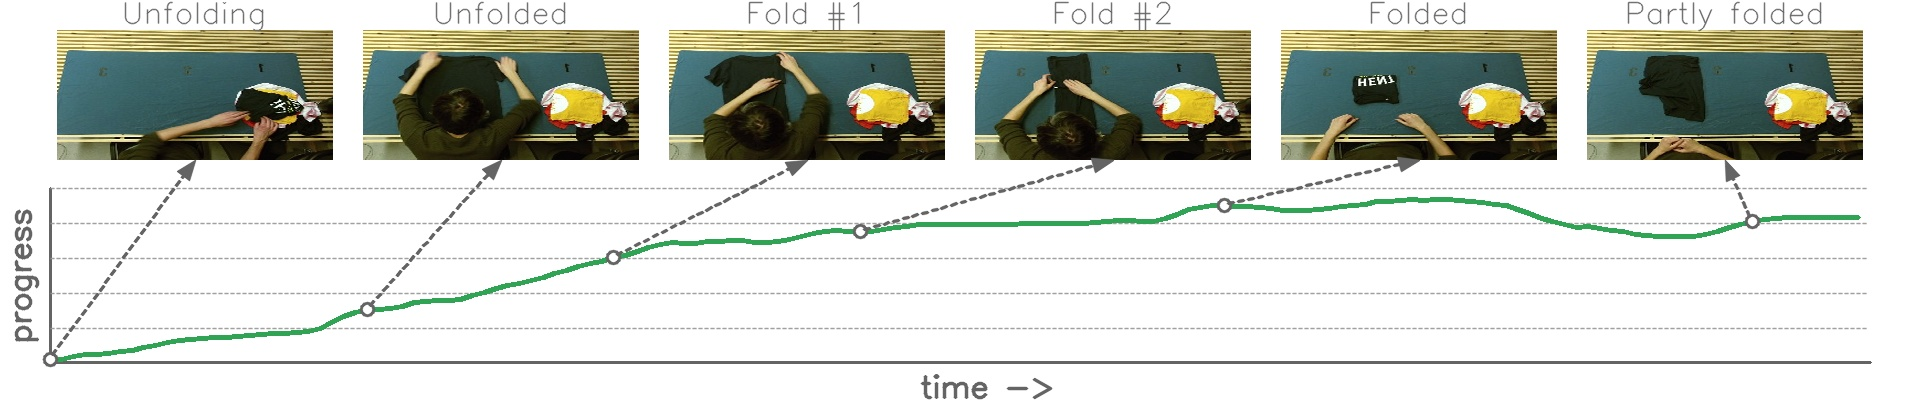
\includegraphics[ width=\linewidth]{figures/figs_cases_paper_reward_plot_1031.jpg}
        \end{minipage}
        \begin{minipage}{0.04\linewidth}
            \caption{}
            \label{fig:casesP1e}
        \end{minipage}
    \end{subfigure}
    \par\medskip

    \begin{subfigure}[b]{\linewidth}
        \begin{minipage}{0.94\linewidth}
            \centering
            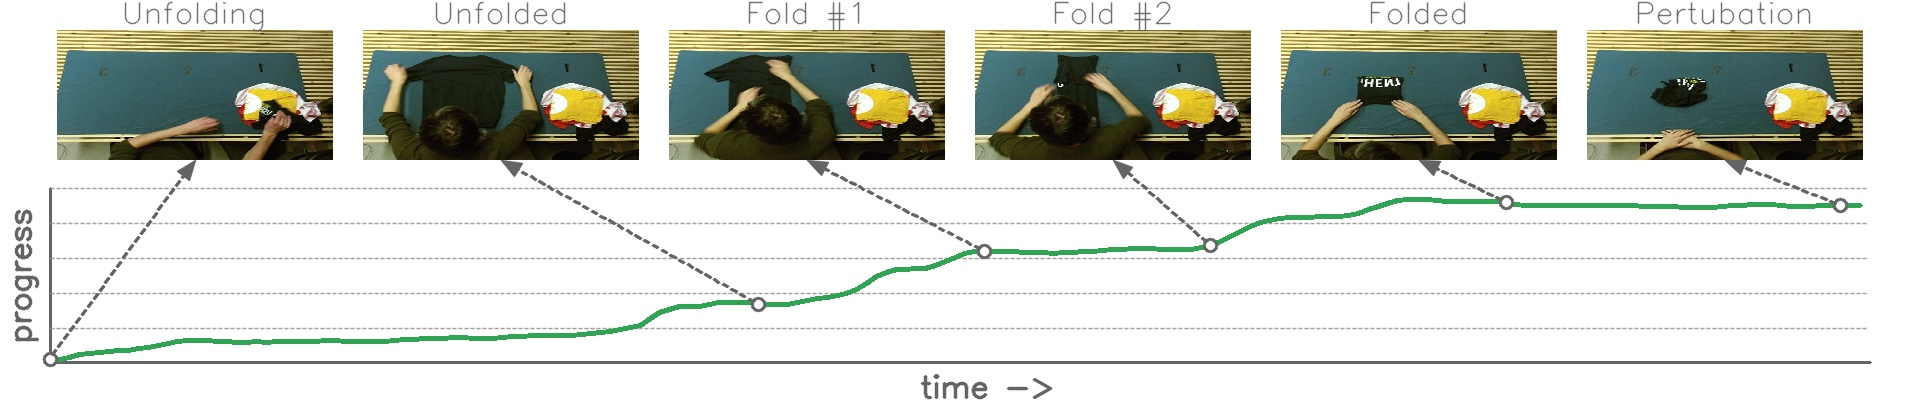
\includegraphics[ width=\linewidth]{figures/figs_cases_paper_reward_plot_1030.jpg}
        \end{minipage}
        \begin{minipage}{0.04\linewidth}
            \caption{}
            \label{fig:casesP1f}
        \end{minipage}
    \end{subfigure}

    \caption{Task progression plots and corresponding images of out-of-sample cases to specifically test properties of the learned process monitoring metrics.}
    \label{fig:casesP2}
\end{figure}


% ===================================================

\section{Conclusion} \label{sec:rewards_conc}
Learning the intention of a task from example demonstrations is an important step for process monitoring in manufacturing systems and reinforcement learning of robotic manipulation skills. In particular, evaluating the progress of folding clothing requires dealing with an infinite amount of states and occlusions caused by deformations.
While state estimation can be done with instrumentation of the cloth (\cref{ch:instrumentation}), the requirement of translating the state to a scalar reward is still required.

In this chapter, we proposed a method to encode task intent by assigning a progression value during task execution. We do this by learning semantically relevant features by using time as a self-supervisory signal on videos with task demonstrations captured from multiple perspectives. We align the resulting embedding to express task progression and task quality. We used our method to demonstrate the first results on expressing task progression for the challenging case of folding clothing. We find that the process monitoring metric assigns correct progression values on meaningful moments during task execution. With case-based examples, we show that our method learns task progression metrics that are invariant to noise, actor morphology and execution speed. An important characteristic is that our approach does not require labelling task progression of existing demonstrations manually. Therefore, our methodology circumvents the need to engineer task progression metrics by learning the task intent from existing task demonstrations. Future work can explore the use of our learned reward function in a \gls{RL} setting, incorporating multiple modalities, using probabilistic embeddings and exploring different loss functions. We discuss these ideas in detail in \cref{subsec:conc_future_tcn}. In the following chapter, we also reflect on future work but from a high-level perspective, based on the experience of conducting the research presented in this book.

\end{document}